\documentclass[a4paper,twoside,openright,makeidx,12pt]{book}
%\usepackage{draftcopy}
%$Id: macro.tex,v 1.10 2004/12/08 13:38:58 acary Exp $


%\usepackage{a4wide}
\textheight 25cm
\textwidth 16.5cm
\topmargin -1cm
%\evensidemargin 0cm
\oddsidemargin 0cm
\evensidemargin0cm
\usepackage{layout}


\usepackage{amsmath}
\usepackage{amssymb}
\usepackage{minitoc}
%\usepackage{glosstex}
\usepackage{colortbl}
\usepackage{hhline}
\usepackage{longtable}

%\usepackage{glosstex}
%\def\glossaryname{Glossary of Notation}
\def\listacronymname{Acronyms}

\usepackage[outerbars]{changebar}\setcounter{changebargrey}{20}
%\glxitemorderdefault{acr}{l}

%\usepackage{color}
\usepackage{graphicx,epsfig}
\graphicspath{{figure/}}
\usepackage[T1]{fontenc}
\usepackage{rotating}

%\usepackage{algorithmic}
%\usepackage{algorithm}
\usepackage{ntheorem}
\usepackage{natbib}


%\renewcommand{\baselinestretch}{2.0}
\setcounter{tocdepth}{2}     % Dans la table des matieres
\setcounter{secnumdepth}{3}  % Avec un numero.



\newtheorem{definition}{Definition}
\newtheorem{lemma}{Lemma}
\newtheorem{claim}{Claim}
\newtheorem{remark}{Remark}
\newtheorem{assumption}{Assumption}
\newtheorem{example}{Example}
\newtheorem{conjecture}{Conjecture}
\newtheorem{corollary}{Corollary}
\newtheorem{OP}{OP}
\newtheorem{problem}{Problem}
\newtheorem{theorem}{Theorem}


\newcommand{\CC}{\mbox{\rm $~\vrule height6.6pt width0.5pt depth0.25pt\!\!$C}}
\newcommand{\ZZ}{\mbox{\rm \lower0.3pt\hbox{$\angle\!\!\!$}Z}}
\newcommand{\RR}{\mbox{\rm $I\!\!R$}}
\newcommand{\NN}{\mbox{\rm $I\!\!N$}}

\newcommand{\Mnn}{\mathcal M^{n\times n}}
\newcommand{\Mnp}[2]{\ensuremath{\mathcal M^{#1\times #2}}}



\newcommand{\Frac}[2]{\displaystyle \frac{#1}{#2}}

\newcommand{\DP}[2]{\displaystyle \frac{\partial {#1}}{\partial {#2}}}

% c++ variables writting
\newcommand{\varcpp}[1]{\textit{#1}}
% itemize
\newcommand{\bei}{\begin{itemize}}
\newcommand{\ei}{\end{itemize}}

\newcommand{\ie}{i.e.}
\newcommand{\eg}{e.g.}
\newcommand{\cf}{c.f.}
\newcommand{\putidx}[1]{\index{#1}\textit{#1}}

\def\Er{{\rm I\! R}}
\def\En{{\rm I\! N}} 
\def\Ec{{\rm I\! C}}
 
\def\zc{\hat{z}}
\def\wc{\hat{w}}

\font\tete=cmr8 at 8 pt
\font\titre= cmr12 at 20 pt 
\font\titregras=cmbx12 at 20 pt

%----------------------------------------------------------------------
%                  Modification des subsubsections
%----------------------------------------------------------------------
\makeatletter
\renewcommand\thesubsubsection{\thesubsection.\@alph\c@subsubsection}
\makeatother

%----------------------------------------------------------------------
%             Redaction note environnement
%----------------------------------------------------------------------
\makeatletter
\theoremheaderfont{\scshape}
\theoremstyle{marginbreak}
\theorembodyfont{\upshape}
%\newtheorem{rque}{\bf Remarque}[chapter]
%\newtheorem{rque1}{\bf \fsc{Remarque}}[chapter] !!! \fsc est une commande french
\newtheorem{ndr1}{\textbf{\textsc{Redaction note}}}[section]

\newenvironment{ndr}%
{%
\tt
%\centerline{---oOo---}
\noindent\begin{ndr1}%
}%
{%
\begin{flushright}%
%\vspace{-1.5em}\ding{111}
\end{flushright}%
\end{ndr1}%
%\centerline{---oOo---}
}

\makeatother

%----------------------------------------------------------------------
%             Redaction note environnement V.ACARY
%----------------------------------------------------------------------
\makeatletter
\theoremheaderfont{\scshape}
\theoremstyle{marginbreak}
\theorembodyfont{\upshape}
%\newtheorem{rque}{\bf Remarque}[chapter]
%\newtheorem{rque1}{\bf \fsc{Remarque}}[chapter] !!! \fsc est une commande french
\newtheorem{ndr1va}{\textbf{\textsc{Redaction note V. ACARY}}}[section]

\newenvironment{ndrva}%
{%
\tt
%\centerline{---oOo---}
\noindent\begin{ndr1va}%
}%
{%
\begin{flushright}%
%\vspace{-1.5em}\ding{111}
\end{flushright}%
\end{ndr1va}%
%\centerline{---oOo---}
}

\makeatother
%----------------------------------------------------------------------
%             Redaction note environnement V.ACARY
%----------------------------------------------------------------------
\makeatletter
\theoremheaderfont{\scshape}
\theoremstyle{marginbreak}
\theorembodyfont{\upshape}
%\newtheorem{rque}{\bf Remarque}[chapter]
%\newtheorem{rque1}{\bf \fsc{Remarque}}[chapter] !!! \fsc est une commande french
\newtheorem{ndr1fp}{\textbf{\textsc{Redaction note F. PERIGNON}}}[section]

\newenvironment{ndrfp}%
{%
\tt
%\centerline{---oOo---}
\noindent\begin{ndr1fp}%
}%
{%
\begin{flushright}%
%\vspace{-1.5em}\ding{111}
\end{flushright}%
\end{ndr1fp}%
%\centerline{---oOo---}
}

\makeatother
%----------------------------------------------------------------------
%                  Chapter head enviroment
%----------------------------------------------------------------------
\newenvironment{chapter_head}
{%
\begin{center}%
-------------------- oOo --------------------\\%
\ \\%
\begin{minipage}[]{14cm}%
\noindent\normalsize\advance\baselineskip-1pt %
}%
{%
\par\end{minipage}%
\ \\%
\ \\%
-------------------- oOo --------------------
\end{center}%
\vspace*{\stretch{1}}%
\clearpage%
\thispagestyle{empty}%
\vspace*{\stretch{1}}%
\minitoc%
\vspace*{\stretch{2}}%
\clearpage%
}

%%% Local Variables: 
%%% mode: latex
%%% TeX-master: "report"
%%% End: 


\includeonly{}
\usepackage{fancyheadings} 
\usepackage{listings}
\lstset{language=[GNU]C++}
% package pour les images des use cases
%\usepackage[dvips]{graphicx}

\pagestyle{fancy} 
\renewcommand{\chaptermark}[1]% 
{\markboth{{Chap-- \thechapter.\ #1}}{}} 
\renewcommand{\sectionmark}[1]% 
{\markright{{\thesection.\ #1}}} 
\setlength{\headrulewidth}{0.5pt} 
\setlength{\footrulewidth}{0.5pt} 
\newcommand{\helv}{% 
\fontfamily{phv}\fontseries{b}\fontsize{9}{11}\selectfont} 
\lhead[\helv \thepage]{\helv \rightmark} 
\rhead[\helv \leftmark]{\helv \thepage} 
\cfoot{Detailed Design Document -- \today}

\makeindex

\begin{document}
\pagestyle{empty}
\renewcommand{\arraystretch}{1.8}

%%%%%%%%%%%%%%%%%%%%%%%%%%%%%%%%%%%%%%%%%%%%%%%%%%%%%%%%%%%%%%%%%%%%%%%%%%%%%%%%%%%%%%%%%%%%%%%%%%%%%%%%%
%\documentclass[titlepage, 12pt]{report}

%\usepackage[dvips]{graphicx}
%\usepackage{graphics}
%\usepackage{amssymb}
%\usepackage{latexsym}


%\begin{document}

\thispagestyle{empty}

\begin{center}

\includegraphics[height=23mm, width=77mm]{figure/siconos.eps}\\
\textsf{European Project IST2001-37172}\\[6cm]
\end{center}

\begin{center}
\huge
\textsf{\textbf{\textit{Detailled Design Document}}}\\[2.5cm]
\end{center}

\large
\begin{center}
\textsf{\textbf{Version :} 0.1}\\
\textsf{\textbf{Status :}  In progress}\\
\textsf{\textbf{Date : } November 25, 2004}\\
\textsf{\textbf{Document Code :} NUMERICS/DDD}\\[5cm]

\end{center}

\normalsize

\begin{flushright}

\includegraphics[scale=0.3]{figure/Logo-INRIA.eps}
\end{flushright}

\clearpage




%\maketitle

%-----------------------------------------------------------------------------%

\normalsize

\begin{center}
  \textsf{\Large Identification}
\end{center}

\noindent\begin{tabular}{|p{0.3\textwidth}|p{0.7\textwidth}|}
\hline
Document Title : & \textsf{Detailled Design Document} \\
Document Code :  & \textsf{NUMERICS/DDD} \\
\hline
\end{tabular}
\textsf{ }\\


\begin{center}
  \textsf{\Large About the document and its author(s)}
\end{center}

\noindent\begin{tabular}{|p{0.3\textwidth}|p{0.7\textwidth}|}
\hline
Nature :& \textsf{This document defines the Detailled Design for Numerics}\\
Language :& \textsf{English}\\
Author(s) :& \textsf{Fr�d�ric DUBOIS, Sh�h�razade NINEB, Jean-Michel BARBIER}\\
\hline
\end{tabular}

\textsf{ }\\

%\newpage

% cartridge current version
\begin{center}
  \textsf{\Large Current Version}
\end{center}
\begin{tabular}{|p{0.3\textwidth}|p{0.7\textwidth}|}
\hline
Date : &\textsf{November 25, 2004}\\
Current version number : &\textsf{0.1}\\ 
Status :&$\bigotimes$ in progress \\
& $\bigcirc$ validated\\
\textit{ }& \hspace{0.5cm} Approved by :\\
\hline
Document change record since last version : &
\begin{minipage}[t]{0.70\textwidth}
  \begin{itemize}
  \item \textsf{First modifications since the empty version} \\
  \end{itemize}
\end{minipage}\\
\hline
\end{tabular}


\textsf{ }\\
\begin{center}
\textbf{Copyright Notice \copyright}\\
This document may not be reproduced (even partially) or communicated to third
parties without the written authorisation of LMGC.
\end{center}


% log of changes  
\pagebreak
\begin{center}
  \textsf{\Large About the document developing process}
\end{center}
\begin{tabular}{|p{0.3\textwidth}|p{0.7\textwidth}|}
\hline
Date of first issue : &\textsf{November 25, 2004}\\
Current version number : &\textsf{0.1}\\ 
Validated by :& \textsf{}\\
\hline
Document change record since last version : &\textsf{First issue} \\
\hline

\end{tabular}

%\end{document}

%%%%%%%%%%%%%%%%%%%%%%%%%%%%%%%%%%%%%%%%%%%%%%%%%%%%%%%%%%%%%%%%%%%%%%%%%%%%%%%%%%%%%%%%%%%%%%%%%%%%%%%%%


\tableofcontents


\pagestyle{fancy}
%---------------------------------------------------------------------%
\clearpage

%---------------------------------------------------------------------%
%---------------------------------------------------------------------%
\newpage
\pagenumbering{arabic}
\chapter{General description}
\label{Sec:DDD-GeneralDescription}
\section{Introduction}
\label{Sec:DDD-Intoduction}
%\section{Purpose of this document}
\label{Sec:SUM-Purpose-Scope}
The purpose of the Software User Manual is to ...


\subsection{Purpose}
\label{Sec:DDD-Purpose}

The \ac{ddd} aims to specify completely the data structures of~\ac{siconos}. This document relies on the global architecture designed in the \ac{add}.
It consists essentially in a class-diagram and a set of constraints on it to eliminate most of its ambiguities. Implementation choices will also be explained and justified here. 


\subsection{Scope}
\label{Sec:DDD-Scope}

This project is a work-package of European project \ac{SICONOS}. \\
Besides the standard features which are required for a software of scientific computing, the objectives of this project are of the following~:
\begin{itemize}
\item To provide a common framework (formalisms and solver tools) for non smooth problems present in various scientific fields : applied Mathematics, Mechanics, Robotics, Electrical networks, etc. 
\item To be able to rely on existing developments. The platform will not re-implement the dedicated tools, which are already used for the modelling of specific systems in various fields, but will provide a framework to their integration.
\item To support exchanges and comparisons of methods between researchers.
\item To disseminate the know-how to other fields of research and industry.
\item To take into account the diversity of users (end users, algorithms developers, framework builders, industrial).
\item To set up standards in terms of modelling of such systems.
\item To ensure software quality by the use of modern software design methods.
\end{itemize}

\subsection{References}
\label{Sec:DDD-References}

\begin{itemize}

\item \textbf{"Guide to the software detailed design and production phase", PSS-05-05, ESA 1995}
\item "Cours de Conduite de Projets Logiciels", Ioannis Parissis, Master 2 Pro GI 2003-2004.
\item "Cours d'Ing\'enirie des mod\`eles", Jean-Marie Favre, Master 2 Pro GI 2003-2004.
\item \ac{add}, April 2004.

\end{itemize}



\subsection{Overview}
\label{Sec:DDD-Overview}

This document specifies in detail the global architecture given in \ac{add}. It contains also development procedures and justifications of implementation choices.


%---------------------------------------------------------------------------%
%\newpage
\section{Project standards, conventions and procedures}
\label{Sec:DDD-ProjectStandards}
%\input{ProjectStandards}

These points are tackled in the \ac{paql}.\\

To summarise it, the main pieces of information are :

\begin{itemize}

\item Design standard~: UML 1.4
\item Documentation standard~: see \ac{adoc}
\item Programming standard~: see \ac{anp}
\item Programming language~: C++
\item Integrated Development environnement~: Eclipse with C++ plugin (CDT).

\end{itemize}
%---------------------------------------------------------------------------%

%---------------------------------------------------------------------%

%\pagenumbering{arabic}
%\section{Introduction}
%\label{Sec:DDD-Intoduction}
%\section{Purpose of this document}
\label{Sec:SUM-Purpose-Scope}
The purpose of the Software User Manual is to ...



%---------------------------------------------------------------------------%
%\newpage
%\section{Project standards, conventions and procedures}
%\label{Sec:DDD-ProjectStandards}
%\input{ProjectStandards}
%---------------------------------------------------------------------------%


%---------------------------------------------------------------------%
%---------------------------------------------------------------------%
\newpage
\chapter{Component design specifications}
\label{Sec:DDD-ComponentDesignSpecifications}
\section{Global class diagrams}
The following schemas (\ref{fig: Class diagram of the platform}, \ref{fig: Class diagram of the XML management} and \ref{fig: Class diagram with the links between the platform and the XML part})  are class diagrams that describe the global architecture of the \ac{siconos} platform.
	\begin{figure}
	\begin{center}
	\includegraphics[scale=1.2, clip]{figure/kernel2.eps}
	\caption{Class diagram of the platform}
	\label{fig: Class diagram of the platform}
	\end{center}
	\end{figure}
	
	\begin{figure}
	\begin{center}
	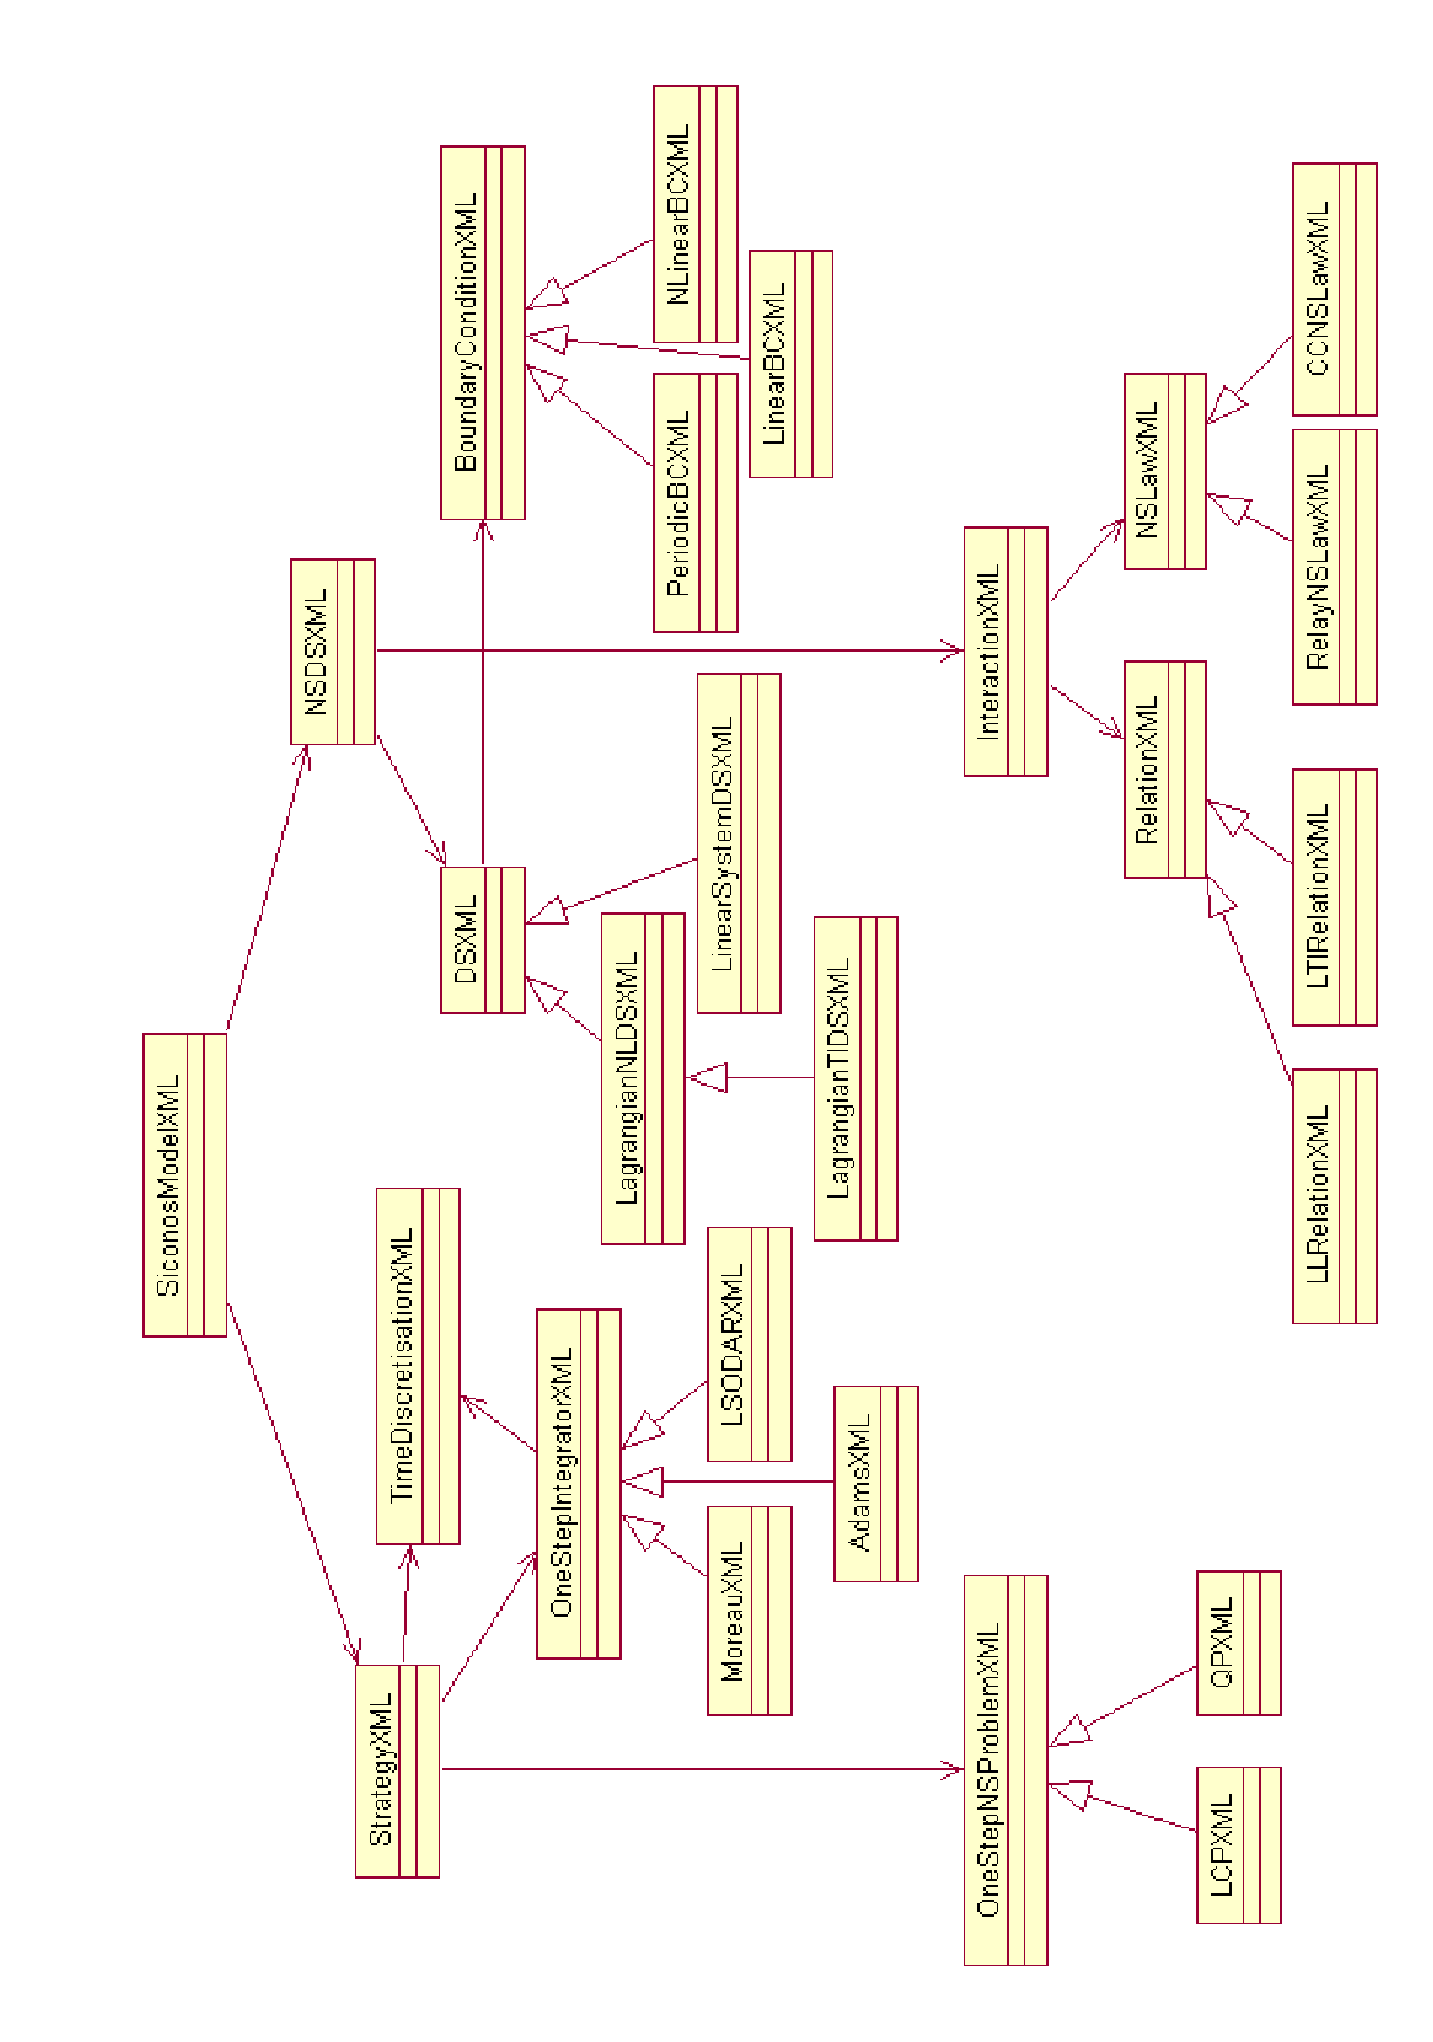
\includegraphics[scale=0.75, clip]{figure/schemaXML.eps}
	\caption{Class diagram of the XML management}
	\label{fig: Class diagram of the XML management}
	\end{center}
	\end{figure}
	
	\begin{figure}
	\begin{center}
	\includegraphics[scale=1.2, clip]{figure/platform.eps}
	\caption{Class diagram with the links between the platform and the XML part}
	\label{fig: Class diagram with the links between the platform and the XML part}
	\end{center}
	\end{figure}


\section{Detailed Design}
\subsection{Code documentation}
\cf~Siconos source code documentation generated by Doxygen

\subsection{Modeling tools update}
The \ref{fig: Class diagram of DSInputOutput and EqualityConstraint added} class diagram represents the EqualityConstraint and DSInputOutput classes (and inherited classes).
	\begin{figure}
	\begin{center}
	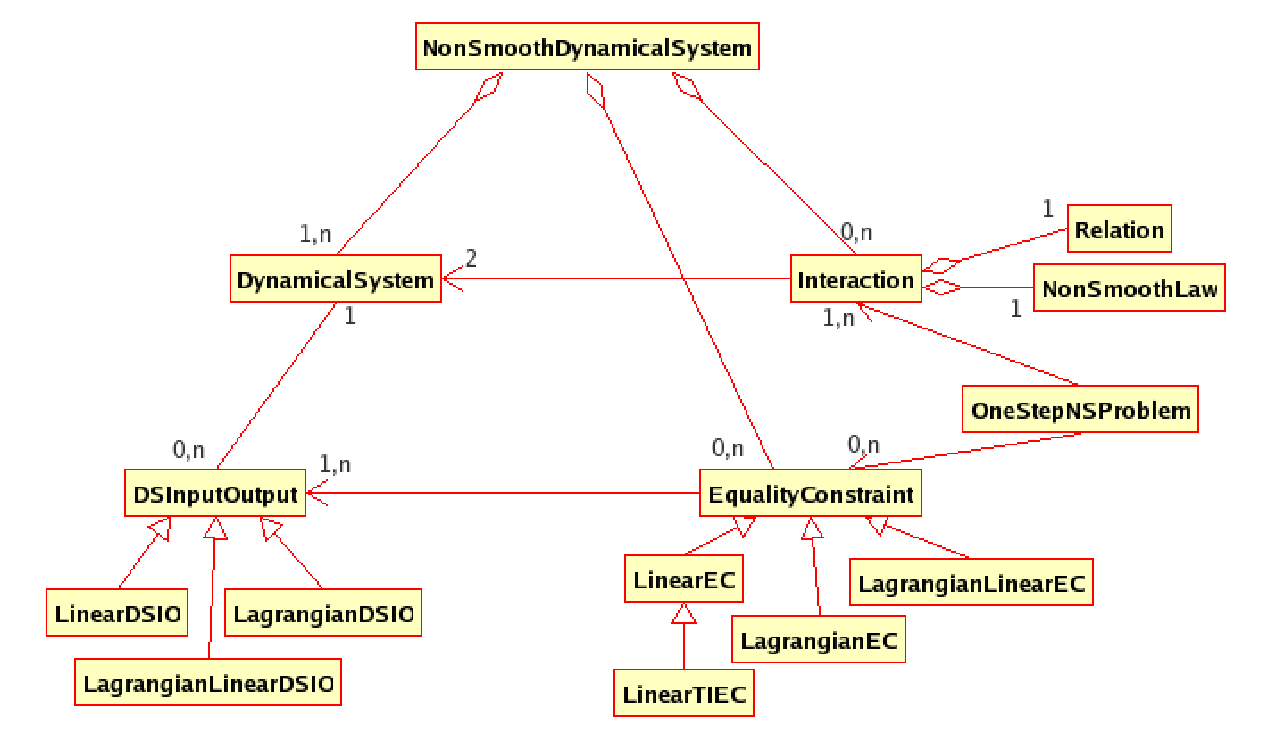
\includegraphics[scale=0.85, clip]{figure/EC.eps}
	\caption{Class diagram of DSInputOutput and EqualityConstraint added}
	\label{fig: Class diagram of DSInputOutput and EqualityConstraint added}
	\end{center}
	\end{figure}
	
\subsubsection{DSInputOutput classes}

\subsubsection{EqualityConstraint classes}



\pagebreak

\section{SiconosMemory}
	
This section explains the global functionning of the class SiconosMemory. This class aims to store some SiconosVectors of previous steps of the simulation.\\
For example, in a Dynamical System, we can save the state of the system. This mechanism is needeed by certain integrators. \\

The attributes of the class are :
\begin{itemize}
\item The maximum number the memory can store.
\item The current number of SiconosVectors stored in the Memory
\item A \acs{stl} vector of pointers on SiconosVector.
\item A pointer on SiconosMemoryXML, used if the memory must be saved in a \ac{xml} file.
\end{itemize} 

The class SiconosMemory is designed to avoid useless copies of SiconosVectors. For the storage of a SiconosVector, there is only one copy : when it enters in the SiconosMemory. Next, the moves of position in the Memory are only done with adresses of pointers. \\
 
We have designed the SiconosMemory to be used preferably with a constant maximum size. In fact, the size is generally known before the initialization of the memory, because each kind of integrator needs a constant number of values of previous steps of the simulation to integrate a system. \\

The management of the relation between SiconosMemory and the \ac{xml} file is the classical one used in the plateform. There are two functions in the SiconosMemory to load or save it in the \ac{xml} DOM tree. The object SiconosMemoryXML realizes this transfer of data.
We chose this method, with a specified \ac{xml} object instead of saving directly the memory with functions in SiconosDOMTreeTools in order to respect the philosophy defined in the global architecture. Only the basic objects of the platform, like numbers, vectors and matrices have not a xml manager. %In fact, if we had chosen to load and save directly the SiconosMemory in the DOM tree, why could we not do the same with eveything ? \\

\begin{figure}[h]
\begin{center}
\includegraphics[scale=0.75, angle=-90, bb=20 40 330 710, clip]{figure/SiconosMemory.ps}
\caption{class diagram of SiconosMemory}
\label{fig: class diagram of SiconosMemory}
\end{center}
\end{figure}

\pagebreak
\section{SiconosVector}

After the first version of the platform, it appeared that the class SiconosVector was not satisfactory. A new version is now implemented with a different approach. An abstract interface represents now the vector and functionnalities it can assume (see \ref{fig: class diagram of SiconosVector}). \\

The class SimpleVector represents basic double vector and is totally in accordance with the interface. Its core is a Lapack double vector (class LaVectorDouble). \\

The class CompositeVector represents compound vectors and is partially in accordance with the interface. Its functionnalities are limited because this class do not contain any data. It only point on other vectors, so certain operations could have hazardous border-effects. In a general way, we recommand to use this vector in :

\begin{itemize}
	\item	left member of affectation (CompositeVector = ...).\\
	
	\item	most-right-possible in operators +, -, /, * with other vectors (the vector is then in strictly read-only mode : Vector = 		... + vector + CompositeVector).
\end{itemize}

\textit{Remember, when a CompositeVector is affected or change by an operation, the vectors it references too.} \\

\begin{figure}[h]
\begin{center}
\includegraphics[scale=0.75, bb=20 570 530 830, clip]{figure/SiconosVector.ps}
\caption{class diagram of SiconosVector}
\label{fig: class diagram of SiconosVector}
\end{center}
\end{figure}

%---------------------------------------------------------------------%
\newpage
%---------------------------------------------------------------------------%
\chapter{XML Management}
\label{Sec:DDD-XMLManagement}
\section{XML Schema}
The data of the XML files we can encounter must respect several rules conforming to the \ac{nsds}
and there resolution. Each objects of the platform have specific attributes which are required
or optional. The schema allows to check a lot of rules that are detailed in the \ac{sum}.
To check each information, the schema regroups the defined attributes in several tags relating to
Model, NSDS, DynamicalSystem, Interaction, Relation and NonSmoothLaw, Strategy, TimeDiscretisation,
OneStepIntegrator, OneStepNSProblem.


\section{XML platform}
The management of the XML input/output is made by a set of classes based on the architecture of the
\ac{siconos} platform.

\subsection{Architecture}
In the software, the XML Management uses a tree structure for the XML objects and a DOM tree where all
the data are stored in memory. Each of these objects is linked to the DOM tree, and each object access
only to the data relating to it.

\subsubsection{The XML Management objects}
The figure \ref{fig: Class diagram of the XML management} \& \ref{fig: Class diagram with the links between the platform and the XML part} shows the
structure of the XML Management platform.
The Model is linked to his SiconosModelXML, the NSDS to his NSDSXML, \dots
So, the XML Management platform give to the \ac{siconos} platform the accessors towards the data of the XML DOM tree.
\subsubsection{The data of the XML}
Each XML object can access to the specific branch of the DOM tree which contains the data relating to
the object of the platform. They give an interface to the platform, to manipulate the information of
the DOM tree.
The data stored in the XML Management platform are only used for input and output but never used during the
computations. That's to say the information of the DOM tree are read when the software is launched (if a XML input file is
defined) and data are stored to the DOM tree a the end of each time step of a simulation.
\subsubsection{SiconosDOMTreeTools}
It is a toolbox to manipulate the data of the platform to store them under XML format.


\subsection{Unfolding of the creation of the platform}
The two ways to construct the platform are using similar mechanisms, and especially the same creating
method.
\subsubsection{XML file loading}
At first, when a XML file is loaded, the data of the file are copied in memory in a DOM tree. From
there, the XML Management platform is built.\\
The SiconosModelXML owns the DOM tree and create NSDSXML and StrategyXML objects. The created objects
only know the branch of the DOM tree relating to them. Gradually, the NSDSXML will create the
different XML objects of the dynamical systems (DSXML, LagrangianNLDSXML, LagrangianTIDSXML,
LinearSystemDSXML), and the different interactions.\\
Then, after all the XML objects have been created, the \ac{siconos} platform is built.\\
The Model which has lead the construction of the XML platform begin the creation of the NSDS,
DynamicalSystem, LagrangianNLDS, ..., Interaction, Relation, ..., NonSmoothLaw, ..., Strategy,
TimeDiscretisation, OneStepIntegrator, Moreau, ..., OneStepNSProblem, LCP and QP by using the
relating XML objects.\\
The construction of each object of the platform is made by calling a
"createXxxxx" method (createModel(...), createNSDS(...), createStrategy(...), ...). One parameter
corresponding to the XML object is enough to give the right data to the platform's object for his
construction.
\subsubsection{Creating the platform without XML input file}
Another way to build the platform is to do it manually.
To do this, each object of the \ac{siconos} platform owns functions designed to create/add the
platform's objects belonging to it. These functions must have in parameters all the required data for
the C++ objects. Here are these methods :
\begin{itemize}
	\item In the Model class :
	\begin{itemize}
		\item createNSDS(attributes required for a NSDS : bool BVP)
		\item createTimeStepping()
		\item createEvenrDriven()
	\end{itemize}
	
	\item In the NSDS class :
	\begin{itemize}
		\item addNonLinearSystemDS(number, n, x0, BasicPlugin:vectorField)
		\item addLinearSystemDS(number, n, x0)
		\item addLagrangianNLDS(number, ndof, q0, velocity0, BasicPlugin:computeMass,
		BasicPlugin:computeFInt, BasicPlugin:computeFExt,
		BasicPlugin:computeJacobianQFInt, BasicPlugin:computeJacobianVelocityFInt,
		BasicPlugin:computeJacobianQQNLInertia,
		BasicPlugin:computeJacobianVelocityQNLInertia, BasicPlugin:computeQNLInertia)
		\item addLagrangianTIDS(number, ndof, q0, velocity0, BasicPlugin:computeMass, BasicPlugin:computeFExt, K, C)
		\item addInteraction(number)
	\end{itemize}
	
	\item In the DynamicalSystem class :
	\begin{itemize}
		\item createLinearBC()
		\item createNLinearBC()
		\item createPeriodicBC()
	\end{itemize}
	
	\item In the Interaction class :
	\begin{itemize}
		\item createLagrangianLinearR()
		\item createLagrangianNonLinearR()
		\item createLinearTIR()
		\item createNewtonImpactLawNSL()
		\item createComplementaryConditionNSL()
		\item createRelayNSL()
	\end{itemize}
	
	\item In the Strategy class :
	\begin{itemize}
		\item createTimeDiscretisation()
		\item addMoreau()
		\item addLsodar()
		\item addAdams()
		\item addLCP()
		\item addQP()
	\end{itemize}
	
\end{itemize}
All these functions are calling the createXxxx(...) function of the object to create.

\subsection{Saving the data of the platform}
The save of the platform's data is lead from the Model. The function which do this job is
"saveToXMLFile". It has several things to do before saving tha data in a XML file :
\begin{itemize}
	\item checkXMLPlatform() : This first function will perfom verifications on the XML Management platform. It checks the
	link between the platform's objects and the XML Management objects. If the XML Management
	platform doesn't exist, it will be created and linked to the objects of the \ac{siconos}
	platform. Otherwise, every link between the platform and the XML Management is checked to ensure
	the availability of the XML platform objects.
	\item savePlatformToXML() : Now, all the objects of the platform are linked to their XML Management object. Therefore,
	it is possible to save the data of the platform to the XML DOM tree. The information
	contained in the platform are saved in the DOM tree by using the specific functions given
	by the XML object.
	\item checkXMLDOMTree() : The data of the DOM tree is up to date. But It is important to check that these data still
	respect the XML schema. 
	\item saveSiconosModelInXMLFile(xmlFile) : The last action to be done is to write the data in memory to a file.
\end{itemize}

\newpage
%---------------------------------------------------------------------------%
\chapter{Model loading, Saving and Validation}
\label{Sec:DDD-ModelLoading}


There are two major ways  to perform the loading of a model, i.e., to provide  the platform with data :
\begin{itemize}
\item Loading a XML data file containing the complete or a part of the model
\item Creating a complete or a part of a model through the various API in C++ or C
\end{itemize}
It might also possible to adopt a mixed strategy to load a model. 


\begin{ndr}
  In all of these case, the question of the validity of a model is  posed. 
What is the validation procedure ?
\end{ndr}

These functionnalities are based on the implementation of two adjoint trees of object classes :
\begin{itemize}
\item The first tree, \texttt{SiconosModel}  is the core of the modelingTools and simulationsTools.
\item The second class tree \texttt{siconosModelXML} is devoted the XML Management and interfaces the external  library which implements the API DOM (libxml2).
\end{itemize}
This choice has been justified by the independance with  the external library of the XML management and the ability to extend easily the I/O for new derived object types. It also avoid the overload of the Kernel source code. Moreover, Kernel objects are functionnal without any link to XML objects.

\begin{ndr}
  Improve the justification of the choice of implementation 
\end{ndr}

In this chapter, we describe the implementation and the technical choices for the management of the input user's data and the creation of the model with these information. Particularly, the following are (must be) defined :
\begin{itemize}
\item Creation of the objects inside the class tree SiconosModel
\item Loading of the SiconosModel objects from the minimal data input
\item Linking of the object with the father and the child in the class tree SiconosModel 
\item Linking and loading of the SiconosModel objects from the SiconosModelXML
\item Creation of the objects inside the class tree SiconosModelXML
\item Loading of the SiconosModel objects from the XML data file
\item Linking of the object with the father and the child in the class tree SiconosModelXML
\item Description of some mixed loading Strategy (recall of the \ac{esd} normally !!) \S \ref{Sec:LoadingStrategy}
\item Save strategy of the SiconosModel tree
\item Save strategy of the SiconosModelXML tree
\item Validation strategy of the SiconosModel tree
\item Validation strategy of the SiconosModelXML tree
\end{itemize}


This first  part of chapter which explains  the model loading form the user poiut of view  must be reported in the \ac{sum}. 

\section{Model Loading Strategy}
\label{Sec:LoadingStrategy}


\subsection{Model loading from an  XML data file}
The reading of the file generate a DOM tree in memory with all the data. After that,  the creation of the SiconosModelXML tree is  based on this DOM tree.  The SiconosModelXML belongs to the SiconosModel object, which is the main object of the platform. From the SiconosModel,  the creation process is launched to build  all of the model. From this point, the Model creates the NSDS, which one creates the dynamical systems, ... The building is "top down" and gradually, with the Model at the top of the platform. 





\subsection{Creating and loading model through the API}
It is also  possible to create the objects of the platform without an XML file by using the API of the platform. The methods given to the users allow the creation of each object of the platform thanks to the constructors of each objects.

\subsection{Mixed strategies}
\label{mixed strategies}
It is possible to create a simulation by loading an XML file and then to add new information in the Kernel.\\
However, the opposite is not recommanded (creating manually some objects, and then loading an XMl file, you would have several SiconosModel in memory).\\
So, by loading some data from an input file, the creation process will build the platform with these data. And then you can manipulate the loaded information and also add dynamical systems, interactions, ...


%\section{Definition of three major types of construtors for the Siconosmodel objects.}
%% \subsection{The "create" methods}
%% The "create" functions have for goal to initialize the relating object. They fill its fields with XML data and link the objects belonging to it to their corresponding XML object, or, if the platform is manually built, only fill its fields with the data given in paramaters.


%In this section, we define three majors types of constructors which must be defined and used in all classes of the platfrom for the creation of objects. In order to fix ideas, we consider a template objects of the form :

 % {\ttfamily \raggedright \small
\#include\ <{}string>{}\\
\#include\ <{}vector>{}\\
\ \\
\ \\
using\ \textbf{namespace}\ std;\\
\ \\
\textbf{class}\ BaseObjectSiconos\ \{\\
\textbf{public}:\\
\ \ \ \ BaseObjectSiconos();\\
\ \ \ \ BaseObjectSiconos(\textbf{int}\ ii);\\
\ \ \ \ \textbf{void}\ display();\\
\ \ \ \ \textbf{void}\ fillObjectWithObjectXML();\\
\ \ \ \ \textbf{void}\ linkObjectXML();\\
\textbf{private}\ :\\
\ \ \textbf{int}\ i;\\
\ \ string\ type;\ \\
\};\\
\ \\
\ \\
\textbf{class}\ CompositionObject\\
\{\\
\ \textbf{public}:\\
\ \ \ \ CompositionObject();\\
\ \ \ \ CompositionObject(\textbf{int}\ ii);\\
\ \ \ \ \textbf{private}\ :\\
\ \ \textbf{int}\ i;\\
\};\\
\ \\
\textbf{class}\ ExternalObject\\
\{\\
\ \textbf{public}:\\
\ \ \ \ ExternalObject();\\
\ \ \ \ ExternalObject(\textbf{int}\ ii);\\
\ \ \ \ \textbf{private}\ :\\
\ \ \textbf{int}\ i;\\
\};\\
\ \\
\textbf{class}\ ObjectSiconosXML\ \\
\{\\
\textbf{public}\ :\\
\ \ \ \ ObjectSiconosXML();\\
\ \\
\textbf{private}\ :\\
\textsl{//\ Built-{}in\ types\ attributes\ (int,\ char,\ float,\ ..)}\\
\ \ \ string\ type;\ \\
\ \ \ \textbf{int}\ att;\\
\};\\
\ \\
\ \\
\textbf{class}\ ObjectSiconos\ :\ BaseObjectSiconos\\
\{\\
\textbf{public}\ :\\
ObjectSiconos();\\
ObjectSiconos(\textbf{int}\ aatt);\\
ObjectSiconos(ObjectSiconosXML\ $\ast$oxml);\\
\textbf{void}\ display();\\
\textbf{void}\ fillObjectWithObjectXML();\\
\textbf{void}\ linkObjectXML();\\
\ \\
\textbf{private}\ :\\
\textsl{//\ Built-{}in\ types\ attributes\ (int,\ char,\ float,\ ..)}\\
\ \ \ \ string\ type;\ \\
\ \ \ \textbf{int}\ att;\\
\ \\
\ \\
\textsl{//\ Objects\ members\ (Composition)}\\
\ \ \ CompositionObject\ compositionObject;\\
\ \\
\ \\
\textsl{//\ Pointer\ on\ external\ objects}\\
\ \ \ ObjectSiconosXML\ $\ast$objectsiconosxml;\\
\ \ \ ExternalObject\ $\ast$externalObject;\\
\ \\
\};\\
\ \\
\ \\
 }
\normalfont\normalsize


%% \begin{lstlisting}[frame=single,caption={Template objects}]
%% Class ObjectSiconos: BaseObjectSiconos
%% {
%% public :
%% ObjectSiconos();
%% ...

%% private :
%% // Built-in types attributes (int, char, float, ..)
%%    string type;
%%    AttType att;
%%    ...

%% // Objects members (Composition)
%%    CompositionObject compositionObject;
%%    ...

%% // Pointer on external objects
%%    ObjectSiconosXML *objectsiconosxml;
%%    ExternalObject *externalObject;
%%    ...
   
%% }
%% \end{lstlisting} 





%\subsection{The Default Constructor}

%The default constructor performs the following operations :
%{\ttfamily \raggedright \small
\#include\ "{}SiconosObject.h"{}\\
\#include\ <{}iostream>{}\\
\ \\
\ \\
ObjectSiconos::ObjectSiconos():\\
\ \ \textsl{//\ Construtors\ of\ the\ Base\ Class}\\
\ \ \ \ BaseObjectSiconos(),\\
\ \ \textsl{//\ Constructors\ of\ the\ Built-{}in\ types}\\
\ \ \ \ type("{}OBJECTSICONOS\underline\ TYPE"{}),att(0),\\
\ \ \textsl{//\ Constructors\ of\ the\ object\ members\ (composition)}\\
\ \ \ \ compositionObject()\\
\{\\
\ \ cout\ <{}<{}\ "{}ObjectSiconos\ -{}-{}\ \textbf{default}\ Constructor"{}\ <{}<{}\ endl;\\
\ \ \\
\ \ \textsl{//\ Initialization\ of\ pointers\ on\ external\ objects}\\
\ \ objectsiconosxml\ =0;\\
\ \ externalObject\ =0;\\
\ \ \\
\ \ \textsl{//\ Do\ we\ need\ to\ call\ the\ new\ operator\ ?}\\
\ \ \textsl{//\ externalObject\ =\ new\ ExternalObject();}\\
\}\\
\ \\
BaseObjectSiconos::BaseObjectSiconos():i(0),type("{}BASE\underline\ TYPE"{})\\
\ \ \ \ \{\ \\
\ \ \ \ \ \ cout\ <{}<{}\ "{}BaseObjectSiconos\ -{}-{}\ \textbf{default}\ Constructor"{}\ <{}<{}\ endl;\\
\ \ \ \ \}\\
\ \\
CompositionObject::CompositionObject():i(0)\\
\ \ \ \ \{\\
\ \ \ \ \};\\
\ \\
ExternalObject::ExternalObject():i(0)\\
\ \ \ \ \{\\
\ \ \ \ \}\\
\ \\
\ \\
 }
\normalfont\normalsize



%% \begin{lstlisting}[frame=single,caption={Default Constructor}]
%% ObjectSiconos::ObjectSiconos() :
%%    // Call explicitely one constructors of the base Object
%%    BaseObjectSiconos(...);
%%    // Call explicitely one constructors of the members
%%    // Built-in types attributes
%%    type("OBJECT_TYPE"), att(defaultvalue),
%%    //Object members :
%%    compositionObject(newDefaultValueIfNeccesary), ...
%%    {
%%    Initialization of pointers on external objects
%%    this->objectsiconosXML = 0 ;  // ObjectXML pointer
%%    this->externalObject = 0;

%%    // Do we need to call the new operator ?
%%     externalObject = new ExternalObject();
%%    }
%% \end{lstlisting} 

%\begin{ndr}
%  \begin{enumerate}
%  \item Remove init() method !!!! This is the role of the Default constructor.
%  \item Do we need to use the new operator if the sizes of the object are not defined ? What is the interest to call the Default constructor with a new ?
%  \end{enumerate}

%\end{ndr}

%\subsection{Constructor with the mininal data}

%This constructor performs  the contruction of a object through given a minimal set of data that corresponds to required data for each created object.  It is composed of the following operations :
%{\ttfamily \raggedright \small
\#include\ "{}SiconosObject.h"{}\\
\#include\ <{}iostream>{}\\
\ \\
ObjectSiconos::ObjectSiconos(\textbf{int}\ aatt,\ string\ ttype):\\
\ \ \textsl{//\ Construtors\ of\ the\ Base\ Class}\\
BaseObjectSiconos(2$\ast$aatt),\\
\ \ \textsl{//\ Constructors\ of\ the\ Built-{}in\ types}\\
type(ttype),att(aatt),\\
\ \ \textsl{//\ Constructors\ of\ the\ object\ members\ (composition)}\\
compositionObject(5$\ast$aatt)\\
\{\\
\ \ cout\ <{}<{}\ "{}ObjectSiconos\ -{}-{}\ Constructor\ with\ minimal\ data"{}\ <{}<{}\ endl;\\
\ \ \textsl{//\ ObjectSiconos();\ //\ Dangerous\ Fix\ the\ order\ ??}\\
\ \ \textsl{//\ Initialization\ of\ pointers\ on\ external\ objects}\\
\ \ objectsiconosxml\ =0;\\
\ \ externalObject\ =\ \textbf{new}\ ExternalObject(aatt);\\
\}\\
\ \\
CompositionObject::CompositionObject(\textbf{int}\ ii):i(ii)\\
\ \ \ \ \{\\
\ \ \ \ \};\\
\ \\
\ \\
ExternalObject::ExternalObject(\textbf{int}\ ii):i(ii)\\
\ \ \ \ \{\\
\ \ \ \ \}\\
\ \\
BaseObjectSiconos::BaseObjectSiconos(\textbf{int}\ ii):i(ii),type("{}BASE\underline\ TYPE"{})\\
\ \ \ \ \{\ \\
\ \ \ \ \ \ cout\ <{}<{}\ "{}BaseObjectSiconos\ -{}-{}\ \textbf{default}\ Constructor"{}\ <{}<{}\ endl;\\
\ \ \ \ \}\\
\ \\
 }
\normalfont\normalsize


%% \begin{lstlisting}[frame=single,caption={Constructor from the mininal data}]
%% Object::object(AttributeType1 data1,...,AttributeTypeN dataN )
%%    {
%%    Object(); // Default constructor

%%    // Loading of Simple type attributes
%%    this->attribute1 = data1 ; //loading of the attributes
%%    ....
%%    this->attributeN = dataN ;

%%    //Object attributes

%%    // if data are present for this object call the specific constructor
%%    attributeObject1 = new AttributeObject1type(data11, data 1N);

%%    // if not, do we need to call the default constructor (new needed ?)
%%    attributeObject1 = new AttributeObject1type();
%%    // XML Management, node creation, and link downwards ? see NDR below
%%    }
%% \end{lstlisting} 

% \begin{ndr}
%   \begin{enumerate}
%   \item Be careful of the conflict between the new in the Default Constructor and in this constructor, if a new is called in the default Constructor
%   \item Define if the object in attributes must created now of after and then link
%   \item Define the procedure for the XML management :
%     \begin{itemize}
%     \item  Where  is the constructor of the assciated ObjectXML ? 
%     \item  Use of the SaveObjectXML ?
%     \item  Creation of XML sub -tree ? Advantages : Don't need to know what is the father node to fullfill a node at the moment of construction
%     \end{itemize}
%   \end{enumerate}
% \end{ndr}


%\section{Constructor with the ObjectXML of the SiconosModelXML tree}\label{xml_constructor}

%This constructor performs  the contruction of a object given a XML node. There is two steps in this type of contruction  based on the two-associated objetcs, i.e, Object, ObjectXML (for instance, DynamicalSystem and DynamicalSystemXML). The first one is the loading of the ObjectXML from the XML node.This step will be detailed in the section \ref{Sec:XMLnode}. The second  step is the loading of the attributes of the object from the ObjectXML. The operations are described in the Listing~\ref{ConstructorObjectXML}.

%{\ttfamily \raggedright \small
\#include\ "{}SiconosObject.h"{}\\
\#include\ <{}iostream>{}\\
\ \\
ObjectSiconos::ObjectSiconos(ObjectSiconosXML\ $\ast$objectsiconosxml):\\
\ \ \textsl{//\ Construtors\ of\ the\ Base\ Class}\\
BaseObjectSiconos(),\\
\ \ \textsl{//\ Constructors\ of\ the\ Built-{}in\ types}\\
type("{}OBJETSICONOS\underline\ TYPE"{}),att(),\\
\ \ \textsl{//\ Constructors\ of\ the\ object\ members\ (composition)}\\
compositionObject()\\
\{\\
\ \ cout\ <{}<{}\ "{}ObjectSiconos\ -{}-{}\ Constructor\ with\ minimal\ data"{}\ <{}<{}\ endl;\\
\ \ \textsl{//\ ObjectSiconos();\ //\ Dangerous\ Fix\ the\ order\ ??}\\
\ \ \textsl{//\ Initialization\ of\ pointers\ on\ external\ objects}\\
\ \\
\ \ objectsiconosxml\ =\ oxml;\\
\ \ \textsl{//\ Loading\ of\ the\ attribute\ from\ the\ ObjectXML}\\
\ \ fillObjectWithObjectXML();\\
\ \ \textsl{//\ Create\ from\ factory\ if\ needed\ (new)\ and\ \ link\ downwards\ the\ External\ objects}\\
\ \ linkObjectXML();\\
\ \\
\}\\
\ \\
 }
\normalfont\normalsize


%% \begin{lstlisting}[frame=single,caption={Constructor from the ObjectXML of the SiconosModelXML tree }, label={ConstructorObjectXML}]
%% Object::Object(ObjectXML objectxml)
%%    {
%%     Object(); // Default constructor
%%     this->objectxml = objectXML;        
%%     this->fillObjectWithDSXML(); // Loading of the attribute from the ObjectXML
%%     this->linkObjectXML();       // Link downwards
%%    }
%% \end{lstlisting} 


%\clearpage

%{\ttfamily \raggedright \small
ObjectSiconos::ObjectSiconos():BaseObjectSiconos(),type("{}DERIVED\underline\ TYPE"{}),att(100),\ compositionObject()\\
\{\\
\ \ cout\ <{}<{}\ "{}ObjectSiconos\ -{}-{}\ default\ Constructor"{}\ <{}<{}\ endl;\\
\ \ objectsiconosxml\ =0;\\
\ \ externalObject\ =0;\\
\}\\
\ \\
\ \\
ObjectSiconos::ObjectSiconos(int\ aatt,\ string\ ttype):BaseObjectSiconos(),type(ttype),att(aatt),\ compositionObject()\\
\{\\
\ \ cout\ <{}<{}\ "{}ObjectSiconos\ -{}-{}\ Constructor\ with\ minimal\ data"{}\ <{}<{}\ endl;\\
\ \ ObjectSiconos();\ \textsl{//\ Fix\ the\ order\ ??}\\
\ \ externalObject\ =\ new\ ExternalObject(aatt);\\
\}\\
\ void\ ObjectSiconos::display()\\
\{\\
\ \ \textsl{//Do\ we\ need\ to\ call\ it\ inside\ the\ braces\ ?}\\
\ \ BaseObjectSiconos::display();\ \\
\ \ cout\ <{}<{}\ this-{}>{}att\ <{}<{}\ endl;\\
\ \ cout\ <{}<{}\ this-{}>{}type\ <{}<{}\ endl;\\
\}\\
\ \\
\ \\
ObjectSiconosXML::ObjectSiconosXML():type("{}TYPE"{}),att(100)\\
\{\\
\}\\
\ \\
\ \\
CompositionObject::CompositionObject():i(0)\\
\ \ \ \ \{\\
\ \ \ \ \};\\
CompositionObject::CompositionObject(int\ ii)\\
\ \ \ \ \{\\
\ \ \ \ \ \ i\ =ii;\\
\ \ \ \ \};\\
\ \\
ExternalObject::ExternalObject():i(0)\\
\ \ \ \ \{\\
\ \ \ \ \}\\
ExternalObject::ExternalObject(int\ ii)\\
\ \ \ \ \{\\
\ \ \ \ \ \ i=\ ii;\\
\ \ \ \ \}\\
\ \\
\ \\
int\ main(void)\\
\ \\
\{\\
\ \\
\ \ ObjectSiconos\ o1;\\
\ \ o1.display();\\
\ \ \\
\ \\
\ \\
\ \ ObjectSiconos\ o2(10,"{}derived\underline\ TYPE"{});\\
\ \ o2.display();\\
\}\\
\ \\
 }
\normalfont\normalsize

{\ttfamily \raggedright \small
\#include\ "{}SiconosObject.h"{}\\
\#include\ <{}iostream>{}\\
\ \\
\ \\
BaseObjectSiconos::BaseObjectSiconos():i(0),type("{}BASE\underline\ TYPE"{})\\
\ \ \ \ \{\ \\
\ \ \ \ \ \ cout\ <{}<{}\ "{}BaseObjectSiconos\ -{}-{}\ default\ Constructor"{}\ <{}<{}\ endl;\\
\ \ \ \ \}\\
void\ BaseObjectSiconos::display()\\
\ \ \ \ \{\\
\ \ \ \ \ \ cout\ <{}<{}\ this-{}>{}i\ <{}<{}\ endl;\\
\ \ \ \ \ \ cout\ <{}<{}\ this-{}>{}type\ <{}<{}\ endl;\\
\ \ \ \ \}\\
\ \\
\ \\
\ \\
ObjectSiconos::ObjectSiconos():BaseObjectSiconos(),type("{}DERIVED\underline\ TYPE"{}),att(100),\ compositionObject()\\
\{\\
\ \ cout\ <{}<{}\ "{}ObjectSiconos\ -{}-{}\ default\ Constructor"{}\ <{}<{}\ endl;\\
\ \ objectsiconosxml\ =0;\\
\ \ externalObject\ =0;\\
\}\\
\ \\
\ \\
ObjectSiconos::ObjectSiconos(int\ aatt,\ string\ ttype):BaseObjectSiconos(),type(ttype),att(aatt),\ compositionObject()\\
\{\\
\ \ cout\ <{}<{}\ "{}ObjectSiconos\ -{}-{}\ Constructor\ with\ minimal\ data"{}\ <{}<{}\ endl;\\
\ \ ObjectSiconos();\ \textsl{//\ Fix\ the\ order\ ??}\\
\ \ externalObject\ =\ new\ ExternalObject(aatt);\\
\}\\
\ void\ ObjectSiconos::display()\\
\{\\
\ \ \textsl{//Do\ we\ need\ to\ call\ it\ inside\ the\ braces\ ?}\\
\ \ BaseObjectSiconos::display();\ \\
\ \ cout\ <{}<{}\ this-{}>{}att\ <{}<{}\ endl;\\
\ \ cout\ <{}<{}\ this-{}>{}type\ <{}<{}\ endl;\\
\}\\
\ \\
\ \\
ObjectSiconosXML::ObjectSiconosXML():type("{}TYPE"{}),att(100)\\
\{\\
\}\\
\ \\
\ \\
CompositionObject::CompositionObject():i(0)\\
\ \ \ \ \{\\
\ \ \ \ \};\\
CompositionObject::CompositionObject(int\ ii)\\
\ \ \ \ \{\\
\ \ \ \ \ \ i\ =ii;\\
\ \ \ \ \};\\
\ \\
ExternalObject::ExternalObject():i(0)\\
\ \ \ \ \{\\
\ \ \ \ \}\\
ExternalObject::ExternalObject(int\ ii)\\
\ \ \ \ \{\\
\ \ \ \ \ \ i=\ ii;\\
\ \ \ \ \}\\
\ \\
\ \\
int\ main(void)\\
\ \\
\{\\
\ \\
\ \ ObjectSiconos\ o1;\\
\ \ o1.display();\\
\ \ \\
\ \\
\ \\
\ \ ObjectSiconos\ o2(10,"{}derived\underline\ TYPE"{});\\
\ \ o2.display();\\
\}\\
\ \\
 }
\normalfont\normalsize

{\ttfamily \raggedright \small
\ \\
\ \\
\ \\
\ \\
\ \\
\ \\
\ \\
\ \\
\ \\
\ \\
\ \\
\ \\
\ \\
\ \\
\ \\
\ \\
\ \\
\#include\ "{}SiconosObject.h"{}\\
\#include\ <{}iostream>{}\\
\ \\
\ \\
BaseObjectSiconos::BaseObjectSiconos():i(0),type("{}BASE\underline\ TYPE"{})\\
\ \ \ \ \{\ \\
\ \ \ \ \ \ cout\ <{}<{}\ "{}BaseObjectSiconos\ -{}-{}\ \textbf{default}\ Constructor"{}\ <{}<{}\ endl;\\
\ \ \ \ \}\\
\textbf{void}\ BaseObjectSiconos::display()\\
\ \ \ \ \{\\
\ \ \ \ \ \ cout\ <{}<{}\ \textbf{this}-{}>{}i\ <{}<{}\ endl;\\
\ \ \ \ \ \ cout\ <{}<{}\ \textbf{this}-{}>{}type\ <{}<{}\ endl;\\
\ \ \ \ \}\\
\ \\
\ \\
\ \\
ObjectSiconos::ObjectSiconos():BaseObjectSiconos(),type("{}DERIVED\underline\ TYPE"{}),att(100),\ compositionObject()\\
\{\\
\ \ cout\ <{}<{}\ "{}ObjectSiconos\ -{}-{}\ \textbf{default}\ Constructor"{}\ <{}<{}\ endl;\\
\ \ objectsiconosxml\ =0;\\
\ \ externalObject\ =0;\\
\}\\
\ \\
\ \\
ObjectSiconos::ObjectSiconos(\textbf{int}\ aatt,\ string\ ttype):BaseObjectSiconos(),type(ttype),att(aatt),\ compositionObject()\\
\{\\
\ \ cout\ <{}<{}\ "{}ObjectSiconos\ -{}-{}\ Constructor\ with\ minimal\ data"{}\ <{}<{}\ endl;\\
\ \ ObjectSiconos();\ \textsl{//\ Fix\ the\ order\ ??}\\
\ \ externalObject\ =\ \textbf{new}\ ExternalObject(aatt);\\
\}\\
\ \textbf{void}\ ObjectSiconos::display()\\
\{\\
\ \ \textsl{//Do\ we\ need\ to\ call\ it\ inside\ the\ braces\ ?}\\
\ \ BaseObjectSiconos::display();\ \\
\ \ cout\ <{}<{}\ \textbf{this}-{}>{}att\ <{}<{}\ endl;\\
\ \ cout\ <{}<{}\ \textbf{this}-{}>{}type\ <{}<{}\ endl;\\
\}\\
\ \\
\ \\
ObjectSiconosXML::ObjectSiconosXML():type("{}TYPE"{}),att(100)\\
\{\\
\}\\
\ \\
\ \\
CompositionObject::CompositionObject():i(0)\\
\ \ \ \ \{\\
\ \ \ \ \};\\
CompositionObject::CompositionObject(\textbf{int}\ ii)\\
\ \ \ \ \{\\
\ \ \ \ \ \ i\ =ii;\\
\ \ \ \ \};\\
\ \\
ExternalObject::ExternalObject():i(0)\\
\ \ \ \ \{\\
\ \ \ \ \}\\
ExternalObject::ExternalObject(\textbf{int}\ ii)\\
\ \ \ \ \{\\
\ \ \ \ \ \ i=\ ii;\\
\ \ \ \ \}\\
\ \\
\ \\
\textbf{int}\ main(\textbf{void})\\
\ \\
\{\\
\ \\
\ \ ObjectSiconos\ o1;\\
\ \ o1.display();\\
\ \ \\
\ \\
\ \\
\ \ ObjectSiconos\ o2(10,"{}derived\underline\ TYPE"{});\\
\ \ o2.display();\\
\}\\
\ \\
 }
\normalfont\normalsize

{\ttfamily \raggedright \small
\ \\
\ \\
\ \\
\ \\
\ \\
\ \\
\ \\
\ \\
\ \\
\ \\
\ \\
\ \\
\ \\
\ \\
\ \\
\ \\
\ \\
\#include\ "{}SiconosObject.h"{}\\
\#include\ <{}iostream>{}\\
\ \\
\ \\
BaseObjectSiconos::BaseObjectSiconos():i(0),type("{}BASE\underline\ TYPE"{})\\
\ \ \ \ \{\ \\
\ \ \ \ \ \ cout\ <{}<{}\ "{}BaseObjectSiconos\ -{}-{}\ \textbf{default}\ Constructor"{}\ <{}<{}\ endl;\\
\ \ \ \ \}\\
\textbf{void}\ BaseObjectSiconos::display()\\
\ \ \ \ \{\\
\ \ \ \ \ \ cout\ <{}<{}\ \textbf{this}-{}>{}i\ <{}<{}\ endl;\\
\ \ \ \ \ \ cout\ <{}<{}\ \textbf{this}-{}>{}type\ <{}<{}\ endl;\\
\ \ \ \ \}\\
\ \\
\ \\
\ \\
ObjectSiconos::ObjectSiconos():BaseObjectSiconos(),type("{}DERIVED\underline\ TYPE"{}),att(100),\ compositionObject()\\
\{\\
\ \ cout\ <{}<{}\ "{}ObjectSiconos\ -{}-{}\ \textbf{default}\ Constructor"{}\ <{}<{}\ endl;\\
\ \ objectsiconosxml\ =0;\\
\ \ externalObject\ =0;\\
\}\\
\ \\
\ \\
ObjectSiconos::ObjectSiconos(\textbf{int}\ aatt,\ string\ ttype):BaseObjectSiconos(),type(ttype),att(aatt),\ compositionObject()\\
\{\\
\ \ cout\ <{}<{}\ "{}ObjectSiconos\ -{}-{}\ Constructor\ with\ minimal\ data"{}\ <{}<{}\ endl;\\
\ \ ObjectSiconos();\ \textsl{//\ Fix\ the\ order\ ??}\\
\ \ externalObject\ =\ \textbf{new}\ ExternalObject(aatt);\\
\}\\
\ \textbf{void}\ ObjectSiconos::display()\\
\{\\
\ \ \textsl{//Do\ we\ need\ to\ call\ it\ inside\ the\ braces\ ?}\\
\ \ BaseObjectSiconos::display();\ \\
\ \ cout\ <{}<{}\ \textbf{this}-{}>{}att\ <{}<{}\ endl;\\
\ \ cout\ <{}<{}\ \textbf{this}-{}>{}type\ <{}<{}\ endl;\\
\}\\
\ \\
\ \\
ObjectSiconosXML::ObjectSiconosXML():type("{}TYPE"{}),att(100)\\
\{\\
\}\\
\ \\
\ \\
CompositionObject::CompositionObject():i(0)\\
\ \ \ \ \{\\
\ \ \ \ \};\\
CompositionObject::CompositionObject(\textbf{int}\ ii)\\
\ \ \ \ \{\\
\ \ \ \ \ \ i\ =ii;\\
\ \ \ \ \};\\
\ \\
ExternalObject::ExternalObject():i(0)\\
\ \ \ \ \{\\
\ \ \ \ \}\\
ExternalObject::ExternalObject(\textbf{int}\ ii)\\
\ \ \ \ \{\\
\ \ \ \ \ \ i=\ ii;\\
\ \ \ \ \}\\
\ \\
\ \\
\textbf{int}\ main(\textbf{void})\\
\ \\
\{\\
\ \\
\ \ ObjectSiconos\ o1;\\
\ \ o1.display();\\
\ \ \\
\ \\
\ \\
\ \ ObjectSiconos\ o2(10,"{}derived\underline\ TYPE"{});\\
\ \ o2.display();\\
\}\\
\ \\
 }
\normalfont\normalsize

{\ttfamily \raggedright \small
\ \\
\ \\
\ \\
\ \\
\ \\
\ \\
\ \\
\ \\
\ \\
\ \\
\ \\
\ \\
\ \\
\ \\
\ \\
\ \\
\ \\
\#include\ "{}SiconosObject.h"{}\\
\#include\ <{}iostream>{}\\
\ \\
\ \\
BaseObjectSiconos::BaseObjectSiconos():i(0),type("{}BASE\underline\ TYPE"{})\\
\ \ \ \ \{\ \\
\ \ \ \ \ \ cout\ <{}<{}\ "{}BaseObjectSiconos\ -{}-{}\ \textbf{default}\ Constructor"{}\ <{}<{}\ endl;\\
\ \ \ \ \}\\
\textbf{void}\ BaseObjectSiconos::display()\\
\ \ \ \ \{\\
\ \ \ \ \ \ cout\ <{}<{}\ \textbf{this}-{}>{}i\ <{}<{}\ endl;\\
\ \ \ \ \ \ cout\ <{}<{}\ \textbf{this}-{}>{}type\ <{}<{}\ endl;\\
\ \ \ \ \}\\
\ \\
\ \\
\ \\
ObjectSiconos::ObjectSiconos():BaseObjectSiconos(),type("{}DERIVED\underline\ TYPE"{}),att(100),\ compositionObject()\\
\{\\
\ \ cout\ <{}<{}\ "{}ObjectSiconos\ -{}-{}\ \textbf{default}\ Constructor"{}\ <{}<{}\ endl;\\
\ \ objectsiconosxml\ =0;\\
\ \ externalObject\ =0;\\
\}\\
\ \\
\ \\
ObjectSiconos::ObjectSiconos(\textbf{int}\ aatt,\ string\ ttype):BaseObjectSiconos(),type(ttype),att(aatt),\ compositionObject()\\
\{\\
\ \ cout\ <{}<{}\ "{}ObjectSiconos\ -{}-{}\ Constructor\ with\ minimal\ data"{}\ <{}<{}\ endl;\\
\ \ ObjectSiconos();\ \textsl{//\ Fix\ the\ order\ ??}\\
\ \ externalObject\ =\ \textbf{new}\ ExternalObject(aatt);\\
\}\\
\ \textbf{void}\ ObjectSiconos::display()\\
\{\\
\ \ \textsl{//Do\ we\ need\ to\ call\ it\ inside\ the\ braces\ ?}\\
\ \ BaseObjectSiconos::display();\ \\
\ \ cout\ <{}<{}\ \textbf{this}-{}>{}att\ <{}<{}\ endl;\\
\ \ cout\ <{}<{}\ \textbf{this}-{}>{}type\ <{}<{}\ endl;\\
\}\\
\ \\
\ \\
ObjectSiconosXML::ObjectSiconosXML():type("{}TYPE"{}),att(100)\\
\{\\
\}\\
\ \\
\ \\
CompositionObject::CompositionObject():i(0)\\
\ \ \ \ \{\\
\ \ \ \ \};\\
CompositionObject::CompositionObject(\textbf{int}\ ii)\\
\ \ \ \ \{\\
\ \ \ \ \ \ i\ =ii;\\
\ \ \ \ \};\\
\ \\
ExternalObject::ExternalObject():i(0)\\
\ \ \ \ \{\\
\ \ \ \ \}\\
ExternalObject::ExternalObject(\textbf{int}\ ii)\\
\ \ \ \ \{\\
\ \ \ \ \ \ i=\ ii;\\
\ \ \ \ \}\\
\ \\
\ \\
\textbf{int}\ main(\textbf{void})\\
\ \\
\{\\
\ \\
\ \ ObjectSiconos\ o1;\\
\ \ o1.display();\\
\ \ \\
\ \\
\ \\
\ \ ObjectSiconos\ o2(10,"{}derived\underline\ TYPE"{});\\
\ \ o2.display();\\
\}\\
\ \\
 }
\normalfont\normalsize







%\subsection{On the use of the operator new and delete in the constructors and the destructors}


%\begin{ndr}
%  \begin{enumerate}
%  \item Define a rule on the use  operator new and delete in the constructors and the destructors. For instance, 
%    \begin{itemize}
%    \item Should we delete objects in the destructor which have been created with a new in a Constructor ?
%    \end{itemize}
%  \item A question, which is also related, is  the use of a pointer rather than directly a object in the attributes of a Object. (Example in DynamicalSystem, difference between x and r ?)
%  \end{enumerate}
%\end{ndr}
%\ac{tbd}
%\clearpage


\section{Object Factories}

\subsection{Purpose}

\subsection{Implementation}

\clearpage



\label{Sec:DDD-XMLLoading}
\clearpage
\section{Definition of three major types of construtors for the SiconosmodelXML objects.}


\subsection{Default constructor}

\begin{verbatim}
ObjectXML::ObjectXML() 
{

}
\end{verbatim}
%\ac{tbd}



\subsection{Constructor from an XML node}


\begin{verbatim}


ObjectXML::ObjectXML( xmlNode* rootNodeOfTheObjectXML ) 
{

}
\end{verbatim}
%\ac{tbd}
\clearpage
\section{Detailed implementation of the Model Loading : Unfolding of the creation of the platform}
The two ways to construct the platform are using similar mechanisms, and especially the same creating
method.



\subsection{Model loading form an XML file}


At first, when a XML file is loaded, the data of the file are copied in memory in a DOM tree. From
there, the XML Management platform is built.\\
The SiconosModelXML owns the DOM tree and create NSDSXML and StrategyXML objects. The created objects
only know the branch of the DOM tree relating to them. Gradually, the NSDSXML will create the
different XML objects of the dynamical systems (DSXML, LagrangianNLDSXML, LagrangianTIDSXML,
LinearSystemDSXML), and the different interactions.\\
Then, after all the XML objects have been created, the \ac{siconos} platform is built.\\
The Model which has lead the construction of the XML platform begin the creation of the NSDS,
DynamicalSystem, LagrangianNLDS, ..., Interaction, Relation, ..., NonSmoothLaw, ..., Strategy,
TimeDiscretisation, OneStepIntegrator, Moreau, ..., OneStepNSProblem, LCP and QP by using the
relating XML objects.\\
The construction of each object of the platform is made by calling a
"createXxxxx" method (createModel(...), createNSDS(...), createStrategy(...), ...). One parameter
corresponding to the XML object is enough to give the right data to the platform's object for his
construction.


\begin{figure}
\begin{center}
        \includegraphics[scale=0.75, clip]{figure/platform_loading_XML.ps}
        \caption{Sequence diagram of the platform's loading with XML file}
        \label{fig: platform's loading1}
\end{center}
\end{figure}

The "create"methods used are partially shown in the diagram \ref{fig: platform's loading1}.







\subsection{Creating a model through the API C++}


The construction of the platform we can see in the diagram \ref{fig: platform's loading2} is lead by an user. The user calls a constructor of the object that he want to create and after that adds the object to the SiconosModel of necessary. For instance, the sequence in the listing \ref{Lst:Creating} can be invoked for creating a model with a DynamicalSystem of the type LagrangianLinearTIDS.
{\ttfamily \raggedright \small
\ \ \textsl{//\ Default\ Constructor\ of\ a\ Model}\\
\ \ Model\ model1;\ \\
\ \ \textsl{//\ Constructor\ of\ a\ nsds\ with\ minimal\ data\ }\\
\ \ NonSmoothDynamicalSystem\ nsds1(\ \textbf{false}\ );\\
\ \ \textsl{//\ Set\ the\ NonSmoothDynamicalSystem\ of\ the\ Model}\\
\ \ model1.setNonSmoothDynamicalSystem(nsds1)\ ;\\
\ \ \ \ \ \ \ \ \\
\ \ SimpleVector\ q0(3);\\
\ \ q0.zero();\ \ q0(0)\ =\ 1.0;\ \ \ \ \ \ \ \ \ \ \ \ \ \ \ \ \\
\ \ SimpleVector\ v0(3);\\
\ \ v0.zero();\ \ \ \ \ \ \ \ \ \ \ \ \ \\
\ \ SiconosMatrix\ mass(3,\ 3);\\
\ \ mass.eye();\\
\ \ SiconosMatrix\ K(3,\ 3);\\
\ \ K.zero();\ \ \ \ \ \ \ \ \ \ \ \ \ \ \ \ \\
\ \ SiconosMatrix\ C(3,\ 3);\\
\ \ C.zero();\\
\ \\
\ \ \textsl{//\ Constructor\ of\ a\ LagrangianLinearTIDS\ with\ minimal\ data\ }\\
\ \ LagrangianLinearTIDS\ lltids1(1,\ 3,\ \&q0,\ \&v0,\ \&mass,\\
\ \ \ \ \ \ \ \ \ \ \ \ \ \ \ \ \ \ \ \ \ \ \ \ \ \ \ \ \ \ \ "{}BasicPlugin:FExt"{},\&K,\ \&C);\\
\ \\
\ \ nsds1.addDS(\&lltids1);\\
\ \\
 }
\normalfont\normalsize


%% \begin{lstlisting}[frame=single, caption={Creating a model through the API C++,label={Lst:Creating}}]
%%   // Default Constructor of a Model
%%   Model model1; 
%%   // Constructor of a nsds with minimal data 
%%   NonSmoothDynamicalSystem nsds1( false );
%%   // Set the NonSmoothDynamicalSystem of the Model
%%   model1.setNonSmoothDynamicalSystem(nsds1) ;
        
%%   SimpleVector q0(3);
%%   q0.zero();  q0(0) = 1.0;                
%%   SimpleVector v0(3);
%%   v0.zero();             
%%   SiconosMatrix mass(3, 3);
%%   mass.eye();
%%   SiconosMatrix K(3, 3);
%%   K.zero();                
%%   SiconosMatrix C(3, 3);
%%   C.zero();

%%   // Constructor of a LagrangianLinearTIDS with minimal data 
%%   LagrangianLinearTIDS lltids1(1, 3, &q0, &v0, &mass,
%%                                "BasicPlugin:FExt",&K, &C);

%%   nsds1.addDS(&lltids1);

%% \end{lstlisting}





 Due to the fact that the destructor of the nsds delete actually the DynamicalSystem which are contained in it, we need to declare a pointer on a DS in  order to avois a doucle delete at the end of the run, see Listing \ref{Lst:Creatingbis}
{\ttfamily \raggedright \small
\ LagrangianLinearTIDS\ $\ast$lltids1;\\
\ \ \textsl{//\ Constructor\ of\ a\ LagrangianLinearTIDS\ with\ minimal\ data\ }\\
\ \ lltids1\ =\ \textbf{new}\ LagrangianLinearTIDS(1,\ 3,\ \&q0,\ \&v0,\ \&mass,\\
\ \ \ \ \ \ \ \ \ \ \ \ \ \ \ \ \ \ \ \ \ \ \ \ \ \ \ \ \ \ \ \ \ \ \ \ \ "{}BasicPlugin:FExt"{},\&K,\ \&C);\\
\ \ nsds1.addDS(lltids1);\\
\ \\
 }
\normalfont\normalsize



%% \begin{lstlisting}[frame=single, caption={Creating a model through the API C++, bis},label={Lst:Creatingbis}]
%%   LagrangianLinearTIDS *lltids1;
%%   // Constructor of a LagrangianLinearTIDS with minimal data 
%%   lltids1 = new LagrangianLinearTIDS(1, 3, &q0, &v0, &mass,
%%                                      "BasicPlugin:FExt",&K, &C);
%%   nsds1.addDS(lltids1);
%% \end{lstlisting}
\begin{ndr}
We need to define precisely a rule for the constructor/destructor with new/delete
\end{ndr}
In the same way,  a complete model may be constructed using the specific constructor of each object. After this operation, we can use either the member function \texttt{setAttributeObject} for pointing or  a member function  \texttt{addAttributeObject} in the case of a vector attribute

 Here are a non exhaustive list of such methods

 \begin{itemize}
 \item In the Model class :
\begin{verbatim}
Model::Model();
Model::setNSDS(NonSmoothDynamicalSystem nsds)
Model::setStrategy(Strategy s)
\end{verbatim}
 \item In the NonSmoothDynamicalSystem class :
\begin{verbatim}
NonSmoothDynamicalSystem::NonSmoothDynamicalSystem(bool BVP)
NonSmoothDynamicalSystem::addDS(DynamicalSystem ds1) // push_back in the vector of pointer on DS
NonSmoothDynamicalSystem::addInteraction(Interaction in1) 
\end{verbatim}  
 \item In the DynamicalSystem class :
\begin{verbatim}
DynamicalSystem::DynamicalSystem(number, n, x0, BasicPlugin:vectorField)
DynamicalSystem::setBC()
\end{verbatim}
 \item In derived class of DynamicalSystem :
\begin{verbatim}
LinearDS::LinearDS(number, n, x0, A)
LagrangianDS::LagrangianDS(number, ndof, q0, velocity0, BasicPlugin:computeMass,
                BasicPlugin:computeFInt, BasicPlugin:computeFExt,
                BasicPlugin:computeJacobianQFInt, BasicPlugin:computeJacobianVelocityFInt,
                BasicPlugin:computeJacobianQQNLInertia,
                BasicPlugin:computeJacobianVelocityQNLInertia, BasicPlugin:computeQNLInertia)
LagrangianLinearTIDS::LagrangianLinearTIDS(number, ndof, q0, velocity0, BasicPlugin:computeMass, BasicPlugin:computeFExt, K, C)
\end{verbatim}

   
          \item In the Interaction class :
\begin{verbatim}
Interaction::Interaction(number)
addDS(DynamicalSystem * dsi )
setRelation(Relation r)
setNSLaw(Relation r)
\end{verbatim}
          \item In the Relation class :
\begin{verbatim}
Relation::Relation(number,BasicPlugin:computeInput,,BasicPlugin:computeOutput)
\end{verbatim}
          \item In the NSLaw class :
\begin{verbatim}
NSLaw::NSLaw()
\end{verbatim}
 \item In the Strategy class :
\begin{verbatim}
 Strategy::Strategy()
 setTimeDiscretisation(TimeDiscretisation td)
 addOneStepIntegrator(OneStepIntegrator osi) 
\end{verbatim}    
\item ....
 \end{itemize}




%%  The unfolding of the building of the platform's architecture is described in the next sequence diagram.
%% \begin{figure}
%% \begin{center}
%%         \includegraphics[scale=0.75, clip]{figure/platform_loading.ps}
%%         \caption{Sequence diagram of the platform's loading without XML file}
%%         \label{fig: platform's loading2}
%% \end{center}
%% \end{figure}


\subsection{Mixed strategies}
This means that the data read in the file are supplemented with information given in the command
program.
In this case, the XML file is similar to the previous case, then the way to create objects of
the platform apart from a XML file will be detailed in the next section.









\clearpage
 \section{Validation of data}
\subsection{XML schema validation}
When a XML file bring the data needed by the platform, either all the data are given by the XML file or only required data. When the file contains partial data, that means it describe at least a SiconosModel with a NSDS (Non Smooth Dynamical System), composed of at least one Dynamical System.

\subsection{Check member functions}



\clearpage
\section{Saving the data of the platform in a XML file}



The save of the platform's data is lead from the Model. The function which do this job is
"saveToXMLFile". It has several things to do before saving tha data in a XML file :
\begin{itemize}
        \item checkXMLPlatform() : This first function will perfom verifications on the XML Management platform. It checks the
        link between the platform's objects and the XML Management objects. If the XML Management
        platform doesn't exist, it will be created and linked to the objects of the \ac{siconos}
        platform. Otherwise, every link between the platform and the XML Management is checked to ensure
        the availability of the XML platform objects.
        \item savePlatformToXML() : Now, all the objects of the platform are linked to their XML Management object. Therefore,
        it is possible to save the data of the platform to the XML DOM tree. The information
        contained in the platform are saved in the DOM tree by using the specific functions given
        by the XML object.
        \item checkXMLDOMTree() : The data of the DOM tree is up to date. But It is important to check that these data still
        respect the XML schema. 
        \item saveSiconosModelInXMLFile(xmlFile) : The last action to be done is to write the data in memory to a file.
\end{itemize}



%---------------------------------------------------------------------%
%---------------------------------------------------------------------%

%% \newpage
%% %---------------------------------------------------------------------------%
%% \chapter{XML Management}
%% \label{Sec:DDD-XMLManagement}
%% \section{XML Schema}
The data of the XML files we can encounter must respect several rules conforming to the \ac{nsds}
and there resolution. Each objects of the platform have specific attributes which are required
or optional. The schema allows to check a lot of rules that are detailed in the \ac{sum}.
To check each information, the schema regroups the defined attributes in several tags relating to
Model, NSDS, DynamicalSystem, Interaction, Relation and NonSmoothLaw, Strategy, TimeDiscretisation,
OneStepIntegrator, OneStepNSProblem.


\section{XML platform}
The management of the XML input/output is made by a set of classes based on the architecture of the
\ac{siconos} platform.

\subsection{Architecture}
In the software, the XML Management uses a tree structure for the XML objects and a DOM tree where all
the data are stored in memory. Each of these objects is linked to the DOM tree, and each object access
only to the data relating to it.

\subsubsection{The XML Management objects}
The figure \ref{fig: Class diagram of the XML management} \& \ref{fig: Class diagram with the links between the platform and the XML part} shows the
structure of the XML Management platform.
The Model is linked to his SiconosModelXML, the NSDS to his NSDSXML, \dots
So, the XML Management platform give to the \ac{siconos} platform the accessors towards the data of the XML DOM tree.
\subsubsection{The data of the XML}
Each XML object can access to the specific branch of the DOM tree which contains the data relating to
the object of the platform. They give an interface to the platform, to manipulate the information of
the DOM tree.
The data stored in the XML Management platform are only used for input and output but never used during the
computations. That's to say the information of the DOM tree are read when the software is launched (if a XML input file is
defined) and data are stored to the DOM tree a the end of each time step of a simulation.
\subsubsection{SiconosDOMTreeTools}
It is a toolbox to manipulate the data of the platform to store them under XML format.


\subsection{Unfolding of the creation of the platform}
The two ways to construct the platform are using similar mechanisms, and especially the same creating
method.
\subsubsection{XML file loading}
At first, when a XML file is loaded, the data of the file are copied in memory in a DOM tree. From
there, the XML Management platform is built.\\
The SiconosModelXML owns the DOM tree and create NSDSXML and StrategyXML objects. The created objects
only know the branch of the DOM tree relating to them. Gradually, the NSDSXML will create the
different XML objects of the dynamical systems (DSXML, LagrangianNLDSXML, LagrangianTIDSXML,
LinearSystemDSXML), and the different interactions.\\
Then, after all the XML objects have been created, the \ac{siconos} platform is built.\\
The Model which has lead the construction of the XML platform begin the creation of the NSDS,
DynamicalSystem, LagrangianNLDS, ..., Interaction, Relation, ..., NonSmoothLaw, ..., Strategy,
TimeDiscretisation, OneStepIntegrator, Moreau, ..., OneStepNSProblem, LCP and QP by using the
relating XML objects.\\
The construction of each object of the platform is made by calling a
"createXxxxx" method (createModel(...), createNSDS(...), createStrategy(...), ...). One parameter
corresponding to the XML object is enough to give the right data to the platform's object for his
construction.
\subsubsection{Creating the platform without XML input file}
Another way to build the platform is to do it manually.
To do this, each object of the \ac{siconos} platform owns functions designed to create/add the
platform's objects belonging to it. These functions must have in parameters all the required data for
the C++ objects. Here are these methods :
\begin{itemize}
	\item In the Model class :
	\begin{itemize}
		\item createNSDS(attributes required for a NSDS : bool BVP)
		\item createTimeStepping()
		\item createEvenrDriven()
	\end{itemize}
	
	\item In the NSDS class :
	\begin{itemize}
		\item addNonLinearSystemDS(number, n, x0, BasicPlugin:vectorField)
		\item addLinearSystemDS(number, n, x0)
		\item addLagrangianNLDS(number, ndof, q0, velocity0, BasicPlugin:computeMass,
		BasicPlugin:computeFInt, BasicPlugin:computeFExt,
		BasicPlugin:computeJacobianQFInt, BasicPlugin:computeJacobianVelocityFInt,
		BasicPlugin:computeJacobianQQNLInertia,
		BasicPlugin:computeJacobianVelocityQNLInertia, BasicPlugin:computeQNLInertia)
		\item addLagrangianTIDS(number, ndof, q0, velocity0, BasicPlugin:computeMass, BasicPlugin:computeFExt, K, C)
		\item addInteraction(number)
	\end{itemize}
	
	\item In the DynamicalSystem class :
	\begin{itemize}
		\item createLinearBC()
		\item createNLinearBC()
		\item createPeriodicBC()
	\end{itemize}
	
	\item In the Interaction class :
	\begin{itemize}
		\item createLagrangianLinearR()
		\item createLagrangianNonLinearR()
		\item createLinearTIR()
		\item createNewtonImpactLawNSL()
		\item createComplementaryConditionNSL()
		\item createRelayNSL()
	\end{itemize}
	
	\item In the Strategy class :
	\begin{itemize}
		\item createTimeDiscretisation()
		\item addMoreau()
		\item addLsodar()
		\item addAdams()
		\item addLCP()
		\item addQP()
	\end{itemize}
	
\end{itemize}
All these functions are calling the createXxxx(...) function of the object to create.

\subsection{Saving the data of the platform}
The save of the platform's data is lead from the Model. The function which do this job is
"saveToXMLFile". It has several things to do before saving tha data in a XML file :
\begin{itemize}
	\item checkXMLPlatform() : This first function will perfom verifications on the XML Management platform. It checks the
	link between the platform's objects and the XML Management objects. If the XML Management
	platform doesn't exist, it will be created and linked to the objects of the \ac{siconos}
	platform. Otherwise, every link between the platform and the XML Management is checked to ensure
	the availability of the XML platform objects.
	\item savePlatformToXML() : Now, all the objects of the platform are linked to their XML Management object. Therefore,
	it is possible to save the data of the platform to the XML DOM tree. The information
	contained in the platform are saved in the DOM tree by using the specific functions given
	by the XML object.
	\item checkXMLDOMTree() : The data of the DOM tree is up to date. But It is important to check that these data still
	respect the XML schema. 
	\item saveSiconosModelInXMLFile(xmlFile) : The last action to be done is to write the data in memory to a file.
\end{itemize}


%---------------------------------------------------------------------%
%---------------------------------------------------------------------%

\newpage
%---------------------------------------------------------------------------%
\chapter{End-User Plugin system}
\label{Sec:DDD-EndUserPluginsystem}
%---------------------------------------------------------------------------------------%
%					section																%
%---------------------------------------------------------------------------------------%
%\section{Introduction}

The goal of the plugin mechanism is to specify the behavior of a dynamical system and relations. Users can use their own computation methods without re-compile the platform.

%---------------------------------------------------------------------------------------%
%					section																%
%---------------------------------------------------------------------------------------%

Plugin is a set of C functions, but compiled with a C++ compiler (\textit{extern "C"} before the header of the function). It must be supplied as a dynamical library, to allow the platform to load it and use its functions.

Parameters and returned values of function of plugins must be C types (no C++ objects or STL containers). \\

For Integrators which use a FORTRAN routine and pass it a plugin function in parameters, a specific method in the integrator class to make the conversions between C and FORTRAN types (use g2f.h features). \\

From platform point of view, plugin functions are pluged on functions pointers (same signature as the plugin function). A plugin function can be used only if it respects strictly a signature of a pointer function supplied by the platform.

%---------------	sub-section		----------------------------------------------------%
\subsection{Dynamical systems plugins}

\subsubsection{class DynamicalSystem}
\begin{verbatim}
void VectorField(int* sizeOfX, double* time, double* xPtr, double* xdotPtr);
void computeJacobianX(int* sizeOfX, double* time, double* xPtr, double* jacobianXPtr);	
\end{verbatim}

\subsubsection{Class LinearSystemDS}
\begin{verbatim}
void computeF(int* sizeOfF, double* fPtr, double* time);	
void computeU(int* sizeOfU, double* uPtr, double* time);
\end{verbatim}

\subsubsection{Class LagrangianDS}
\begin{verbatim} 
void computeMass(int* sizeOfq, double* time, double* qPtr, double* massPtr);	
void computeFInt(int* sizeOfq, double* time, double* qPtr, double* velocityPtr,
double* fIntPtr);
void computeFExt(int* sizeOfq, double* time, double* qPtr, double* fExtPtr);
void computeQNLInertia(int* sizeOfq, double* qPtr, double* velocityPtr,
double* QNLInertiaPtr);	
void computeJacobianQFInt(int* sizeOfq, double* time, double* qPtr, double* velocityPtr, 
double* jacobPtr);
void computeJacobianVelocityFInt(int* sizeOfq, double* time, double* qPtr, 
double* velocityPtr, double* jacobPtr);
void computeJacobianQQNLInertia(int* sizeOfq, double* qPtr, double* velocityPtr, 
double* jacobPtr);
void computeJacobianVelocityQNLInertia(int* sizeOfq, double* qPtr, double* velocityPtr, 
double* jacobPtr);
\end{verbatim}

%---------------	sub-section		----------------------------------------------------%
\subsection{Relations plugins}

\subsubsection{Class Relation}
\begin{verbatim}
void computeOutput(double* xPtr, double* time, double* lambdaPtr, double* yPtr);
void computeInput(double* xPtr, double* time, double* lambdaPtr, double* rPtr);
\end{verbatim}

\subsubsection{Class LagrangianNonLinearR}
\begin{verbatim}
void computeJacobian(int* sizeOfQ, double* qPtr, int* sizeOfY, double* jacobPtr);	
void computeH(int* sizeOfQ, double* qPtr, int* sizeOfY, double* yPtr);
\end{verbatim}

%---------------	sub-section		----------------------------------------------------%
\subsection{Matrices representation}

Platform and plugin functions are coded in C/C++, but double pointers representing vectors and matrices given in parameters are column-oriented (FORTRAN format), in order to be used simply with FORTRAN computation libraries, e.g. Blas. \\

This is an example : \\

\[M=\left(
\begin{array}{cccc}
1 & 2 & 3 & 4 \\
5 & 6 & 7 & 8 \\
9 & 10 & 11 & 12 \\
\end{array}
\right)\]

n = 3 and m = 4 (indices start at 0 in C language). \\

MFor is the array in memory representing M. Its elements are sorted as follows :

\begin{tabular}[h]{|c|c|c|c|c|c|c|c|c|c|c|c|}
\hline
%\multicolumn{3}{|c|}
1 & 5 & 9 & 2 & 6 & 10 & 3 & 7 & 11 & 4 & 8 & 12 \\
\hline 
\end{tabular} \\

To access to element Mij of matrix M, we need to compute its position in the array : MFor[i + jn].
For example, this is a short C function which returns a M element form its coordinates in the matrix :

\begin{verbatim}
int getMatrixElement(int i, int j, int n, int m, int MFor[])
{
        // i and j are the coordinates of the element in the matrix M
        // n is the number of lines of M
        // m is the number of columns of M
        // MFor is the array representing the matrix M
	
        return MFor[i + j * n];	
}
\end{verbatim}

If we try to get the element $M_{1,3}$ :
\begin{verbatim}
printf("searched element is : \%d", getMatrixElement(1, 3, 3, 4, MFor));
\end{verbatim}

The result displayed on the screen is : \textsf{searched element is : 8}.\\

%---------------------------------------------------------------------------------------%
%					section																%
%---------------------------------------------------------------------------------------%
\section{"False"plugin}
False plugin system allows an integrateur dedicated to a dynamical systems class to integrate its derivated classes too. For example :

\begin{itemize}

\item class DynamicalSystem \\
system : 
\begin{displaymath} \dot x = f(x, t) \end{displaymath} 
\begin{displaymath} \nabla_x f(x, t) \end{displaymath} 


f is a plugin function and is plugged to vectorField function pointer to the platform.
$ \nabla_x f$ is a plugin function and is plugged to computeJacobianX function pointer to the platform. \\

\item  Integrator I, dedicated to integration of systems represented by Dynamicalsystem class.  

\item Class LinearDS, specializes DynamicalSystem class. \\
syst�m :
\begin{displaymath} \dot x = Ax \end{displaymath} 
\begin{displaymath} \nabla_x f(x, t) \end{displaymath} 

\begin{displaymath} f(x, t) = Ax \end{displaymath} 
\begin{displaymath} \nabla_x f(x, t) = A \end{displaymath} 

Functions f and $\nabla_x f $ are in this case very simple and directly supplied by internal methods of LinearDS class. These methods are plugged to the platform during the initialisation phase instead of plugin functions.

\end{itemize}

During the integration, integrator I dedicated to DynamicalSystem class calls f et $\nabla_x f $ functions during computation. It can therefore integrate a LinerDS object since required functions are supplied by the class and respect plugin functions signatures.

In a general manner, every class derivated from another which uses plugin system must use plugin functions too, or supply internal functions which can be plugged instead.

%\begin{ndr} 
%Ajouter un sch�ma ? \\
%\end{ndr}

\begin{figure}[h]
\begin{center}
\includegraphics[scale=0.40]{figure/Plugin.ps}
\caption{General diagram of false plugin mechanism}
\label{fig: General diagram of false plugin mechanism}
\end{center}
\end{figure}


%---------------------------------------------------------------------------------------%
%					section																%
%---------------------------------------------------------------------------------------%
\section{\acs{lmgc90} plugin}
\subsection{Integration into the \acs{kernel}}
This plugin is designed to give specific data required by \acs{kernel} to make a simulation with complex contact detection.
It makes low level computations for the \acs{kernel} to be able to do simulation steps.

\subsection{Data communications}
Data transmission is bidirectionnal between \acs{kernel} and \acs{lmgc90} plugin.\\
The \acs{kernel} needs modeling data supplied by the plugin in modeling phase. Moreover the plugin gives data at the beginning of each steps of the simulation to for the \acs{kernel} to have the good data to make simulation computations.\\
In the other way, the plugin receive informations at the end of each time step as an update of the state of the system.

\subsection{Data to send}
\begin{itemize}
	\item Data loading from \acs{lmgc90} model, to the \acs{kernel} :\\
	number of dynamical systems\\
	q and q dot for each dynamical system\\
	M matrix\\
	Fext at each step\\
	blocking constraints\\
	
	\item Update of the \acs{lmgc90} model :\\
	q and q dot\\
	reaction forces\\
\end{itemize}

%---------------------------------------------------------------------------------------%
%					section																%
%---------------------------------------------------------------------------------------%
\section{Example of a plugin development}

%---------------	sub-section		----------------------------------------------------%
\subsection{Header file}

\textbf{This file is not compulsory in C.}

This is a template of plugin header file, named \textit{plugin\_example.h}:

\begin{verbatim}
#ifndef _PLUGIN_EXAMPLE_
#define _PLUGIN_EXAMPLE_

// decalration of functions of the plugin
extern "C" 
{
	void function1(...);
	...
	void functionN(...);	 
}
#endif //_PLUGIN_EXAMPLE_
\end{verbatim}

%---------------	sub-section		----------------------------------------------------%
\subsection{Source file}

This is the plugin source file, named \textit{plugin\_example.C}:

\begin{verbatim}
#include "plugin_example.h" // if it exists
#include ...

// impl�mentation of plugin functions
extern "C"
{ 
        void function1(...)
        {
                ...
        }

        ...

        void functionN(...)
        {
                ...	 
        }
}
\end{verbatim}

%---------------	sub-section		----------------------------------------------------%
\subsection{Compilation and creation of the dynamic library.}

To build the plugin under Linux (or UNIX), follow the instructions : \\

First, the C file have to be built :
\begin{verbatim}
g++ -g -fbounds-check -w -Wno-deprecated -fPIC -c plugin_example.C
\end{verbatim}

This operation creates a file plugin\_example.o if there are no compilation errors.

\begin{verbatim}
g++ -g -fbounds-check -w -Wno-deprecated -fPIC -shared -W -O plugin_example.C 
-o plugin_example.so
\end{verbatim}

This operation creates the dynamical library plugin\_example.so. Plug-in is ready to use.

%---------------	sub-section		----------------------------------------------------%
\subsection{Plugin and XML file.}

%\begin{ndr} 
%un paragraphe sur le mode de branchement des plugin via le XML ?
%\end{ndr}

Let's take an example. we imagine "function1" of our previous plugin example is used for computing the mass matrix of a non linear Lagrangian system (LagrangianNLDS class of the platform) : we have to indicate to the platform that for the system we want to simulate, computing mass function which is used is function1 of the plugin plugin\_example.
(for more explanations about XML Input data, you can read \ac{sum}) \\

\begin{verbatim}
<DS number='1' type="LagrangianNLDS">
        <Id> DS1 </Id>
        ...	
        <M matrixPlugin="plugin_example:function1"/>
        ...
</DS>
\end{verbatim}


The platform can load the plugin\_example library during the execution only if it knows the path of the plugin on the computer. There are two cases :

\begin{itemize}

\item plugin\_example library.so is in the same repertory as platform exe file : it should work directly.

\item plugin\_example library.so is not in the same repertory as platform exe file : its access path must be added in environment variable LB\_LIBRARY\_PATH. Platform will seek the plugin in this specified path. This is an example of command line to set LB\_LIBRARY\_PATH :



\begin{verbatim}
setenv LD_LIBRARY_PATH /your_path/plugin_example/:$LD_LIBRARY_PATH
\end{verbatim}
\end{itemize}


\newpage
%---------------------------------------------------------------------------%
\chapter{Expert-User Plugin system}
\label{Sec:DDD-ExpertUser-Pluginsystem}
\ac{tbd}
\section{Plug-in Architecture}
\subsection{Factories,registration, dynamically loading of code ....}

\newpage
%---------------------------------------------------------------------------%
\chapter{Python interface}
\label{Sec:DDD-pyInterface}
%---------------------------------------------------------------------------------------%
%					section						%
%---------------------------------------------------------------------------------------%

This chapter reports the development of the Python Interface for the Kernel.

\section{C++ - Python wrapper choice}

There mainly exists two free tools to wrap C++ code with python : Swig and Boost. \\ 

%---------------	sub-section		----------------------------------------------------%

\subsection{Swig}

SWIG is a software development tool that connects programs written in C and C++ with a variety of high-level programming languages. SWIG is used with different types of languages including common scripting languages such as Perl, Python, Tcl/Tk and Ruby (http://www.swig.org). 

The main task to connect C++ with Python using SWIG is to write an interface file. It references the header files that must be wrap and some types declarations for the data strctures that cannot be directly and automatically wrapped.

SWIG is really easy to use, but does not support comnpletely every features of advanced C++ :
\begin{itemize}
\item friend functions
\item overloaded operators with the same number of parameters and close types (int / double, etc.).
\end{itemize}

\subsection{Boost}

Boost is a complete framework for C++ which provides advanced features and completes the Standard Template Library. Its Python wrapper is only one functionnality among many others.

for the developement of the Kernel Python interface, we have chosen SWIG because this tool is easier to use and using Boost just for wrapping C++ with Python seemed not an appropriate solution.


\section{Kernel wrapping}

Connecting the Kernel with Python was pretty fast. We only encountered a problem with down-casting operations. In the kernel, we have STL containers of pointers. For example, an NSDS stores the dynamical systems, but does not know their specific types. So we can access to the specific data of a type of dynamical system after a down-casting operation (static\_cast and dynamic\_cast in C++). This operation is not allowed in Python. To solve this problem, we wrote a cast method in each class which is not a base class. This method wraps the C++ operator of dynamic casting and returns a pointer on the class.\\

The connection of STL containers is not completely automatic. We have to define a Python type for each data type stored in such a container. This type definition must be placed in the interface file. For example, to be able to use a container of pointers on Dynamical systems, we add this command in the Swig interface file: 
\begin{verbatim}
%include "std_vector.i";
namespace std {
    %template(dsVector) vector<DynamicalSystem*>;
}
\end{verbatim}



\section{Miscelleanous}

In the last versions of Swig (1.3.23, 1.3.24), a bug makes fail the compilation of the interface. This is a simple syntax error and we wrote a bash script to correct this. This bug should be fixed soon in Swig distributions.

%---------------------------------------------------------------------%
%---------------------------------------------------------------------%
%\newpage
%\appendix
%\chapter{Source code listing}
%\label{Sec:DDD-SourceCodeListing}
%\section{section 1}

%---------------------------------------------------------------------%


%---------------------------------------------------------------------%
%---------------------------------------------------------------------%
\newpage
\chapter{Software deliverables architecture}
\label{Sec:DDD-SoftwareDeliverablesArchitecture}
%\documentclass[a4paper,twoside,openright,makeidx,12pt]{book}

%%$Id: macro.tex,v 1.10 2004/12/08 13:38:58 acary Exp $


%\usepackage{a4wide}
\textheight 25cm
\textwidth 16.5cm
\topmargin -1cm
%\evensidemargin 0cm
\oddsidemargin 0cm
\evensidemargin0cm
\usepackage{layout}


\usepackage{amsmath}
\usepackage{amssymb}
\usepackage{minitoc}
%\usepackage{glosstex}
\usepackage{colortbl}
\usepackage{hhline}
\usepackage{longtable}

%\usepackage{glosstex}
%\def\glossaryname{Glossary of Notation}
\def\listacronymname{Acronyms}

\usepackage[outerbars]{changebar}\setcounter{changebargrey}{20}
%\glxitemorderdefault{acr}{l}

%\usepackage{color}
\usepackage{graphicx,epsfig}
\graphicspath{{figure/}}
\usepackage[T1]{fontenc}
\usepackage{rotating}

%\usepackage{algorithmic}
%\usepackage{algorithm}
\usepackage{ntheorem}
\usepackage{natbib}


%\renewcommand{\baselinestretch}{2.0}
\setcounter{tocdepth}{2}     % Dans la table des matieres
\setcounter{secnumdepth}{3}  % Avec un numero.



\newtheorem{definition}{Definition}
\newtheorem{lemma}{Lemma}
\newtheorem{claim}{Claim}
\newtheorem{remark}{Remark}
\newtheorem{assumption}{Assumption}
\newtheorem{example}{Example}
\newtheorem{conjecture}{Conjecture}
\newtheorem{corollary}{Corollary}
\newtheorem{OP}{OP}
\newtheorem{problem}{Problem}
\newtheorem{theorem}{Theorem}


\newcommand{\CC}{\mbox{\rm $~\vrule height6.6pt width0.5pt depth0.25pt\!\!$C}}
\newcommand{\ZZ}{\mbox{\rm \lower0.3pt\hbox{$\angle\!\!\!$}Z}}
\newcommand{\RR}{\mbox{\rm $I\!\!R$}}
\newcommand{\NN}{\mbox{\rm $I\!\!N$}}

\newcommand{\Mnn}{\mathcal M^{n\times n}}
\newcommand{\Mnp}[2]{\ensuremath{\mathcal M^{#1\times #2}}}



\newcommand{\Frac}[2]{\displaystyle \frac{#1}{#2}}

\newcommand{\DP}[2]{\displaystyle \frac{\partial {#1}}{\partial {#2}}}

% c++ variables writting
\newcommand{\varcpp}[1]{\textit{#1}}
% itemize
\newcommand{\bei}{\begin{itemize}}
\newcommand{\ei}{\end{itemize}}

\newcommand{\ie}{i.e.}
\newcommand{\eg}{e.g.}
\newcommand{\cf}{c.f.}
\newcommand{\putidx}[1]{\index{#1}\textit{#1}}

\def\Er{{\rm I\! R}}
\def\En{{\rm I\! N}} 
\def\Ec{{\rm I\! C}}
 
\def\zc{\hat{z}}
\def\wc{\hat{w}}

\font\tete=cmr8 at 8 pt
\font\titre= cmr12 at 20 pt 
\font\titregras=cmbx12 at 20 pt

%----------------------------------------------------------------------
%                  Modification des subsubsections
%----------------------------------------------------------------------
\makeatletter
\renewcommand\thesubsubsection{\thesubsection.\@alph\c@subsubsection}
\makeatother

%----------------------------------------------------------------------
%             Redaction note environnement
%----------------------------------------------------------------------
\makeatletter
\theoremheaderfont{\scshape}
\theoremstyle{marginbreak}
\theorembodyfont{\upshape}
%\newtheorem{rque}{\bf Remarque}[chapter]
%\newtheorem{rque1}{\bf \fsc{Remarque}}[chapter] !!! \fsc est une commande french
\newtheorem{ndr1}{\textbf{\textsc{Redaction note}}}[section]

\newenvironment{ndr}%
{%
\tt
%\centerline{---oOo---}
\noindent\begin{ndr1}%
}%
{%
\begin{flushright}%
%\vspace{-1.5em}\ding{111}
\end{flushright}%
\end{ndr1}%
%\centerline{---oOo---}
}

\makeatother

%----------------------------------------------------------------------
%             Redaction note environnement V.ACARY
%----------------------------------------------------------------------
\makeatletter
\theoremheaderfont{\scshape}
\theoremstyle{marginbreak}
\theorembodyfont{\upshape}
%\newtheorem{rque}{\bf Remarque}[chapter]
%\newtheorem{rque1}{\bf \fsc{Remarque}}[chapter] !!! \fsc est une commande french
\newtheorem{ndr1va}{\textbf{\textsc{Redaction note V. ACARY}}}[section]

\newenvironment{ndrva}%
{%
\tt
%\centerline{---oOo---}
\noindent\begin{ndr1va}%
}%
{%
\begin{flushright}%
%\vspace{-1.5em}\ding{111}
\end{flushright}%
\end{ndr1va}%
%\centerline{---oOo---}
}

\makeatother
%----------------------------------------------------------------------
%             Redaction note environnement V.ACARY
%----------------------------------------------------------------------
\makeatletter
\theoremheaderfont{\scshape}
\theoremstyle{marginbreak}
\theorembodyfont{\upshape}
%\newtheorem{rque}{\bf Remarque}[chapter]
%\newtheorem{rque1}{\bf \fsc{Remarque}}[chapter] !!! \fsc est une commande french
\newtheorem{ndr1fp}{\textbf{\textsc{Redaction note F. PERIGNON}}}[section]

\newenvironment{ndrfp}%
{%
\tt
%\centerline{---oOo---}
\noindent\begin{ndr1fp}%
}%
{%
\begin{flushright}%
%\vspace{-1.5em}\ding{111}
\end{flushright}%
\end{ndr1fp}%
%\centerline{---oOo---}
}

\makeatother
%----------------------------------------------------------------------
%                  Chapter head enviroment
%----------------------------------------------------------------------
\newenvironment{chapter_head}
{%
\begin{center}%
-------------------- oOo --------------------\\%
\ \\%
\begin{minipage}[]{14cm}%
\noindent\normalsize\advance\baselineskip-1pt %
}%
{%
\par\end{minipage}%
\ \\%
\ \\%
-------------------- oOo --------------------
\end{center}%
\vspace*{\stretch{1}}%
\clearpage%
\thispagestyle{empty}%
\vspace*{\stretch{1}}%
\minitoc%
\vspace*{\stretch{2}}%
\clearpage%
}

%%% Local Variables: 
%%% mode: latex
%%% TeX-master: "report"
%%% End: 


%\begin{document}
%\pagestyle{empty}
%\renewcommand{\arraystretch}{1.8}



Two deliverables will be distributed, corresponding to the two main uses of the platform~: a basic one for end-users, with only binaries, and a complete one with source files, to allow users to develop news functionalities for the software.

The file names and repertories of the platform core are written in small letters whereas user files have only their first letter in capitals. \\

\section{Expert users distribution}
\label{dudev}

The software \textit{siconos} will be a set of C++ libraries driven by a main program. This kind of libraries are named in the following as "internal libraries" (i.e. libraries developed in \ac{siconos}, in opposition to the "external libraries" which are for example libXML2 or Lapack++). \\

In this distribution, the root directory is named \textit{SICONOS/}. It contains the following sub-directories and files : 
\begin{itemize}

\item  \textit{config/} : contains the configuration files needed by the platform. The sub-dir \textit{xmlschema} holds schema of \ac{xml} files.

\item  \textit{doc/} : contains the \ac{um} in a pdf file \textit{siconos.pdf}. The sub-dir \textit{api} holds the documentation of the internal libraries in html pages generated by Doxygen.

\item \textit{ext/} : contains external libraries (like libXML2) needed by the platform (if the user has not already installed them on his computer).

\item \textit{include/} : contains header files of internal libraries.

\item \textit{lib/} : contains the internal libraries. If a library XXXX is dynamic, the file corresponding is libXXXX.so. If a library XXXX is static, the file corresponding is libXXXX.a.

\item \textit{sample/} : examples of uses of the platform.

\item \textit{siconos/} : contains the binary file \textit{siconos} and its source file \textit{siconos.cpp}. This binary permits to launch a simulation.

\item \textit{src/} : contains the source files of the internal libraries classified by module. For each module, there is a directory, with a Makefile to compile sources and tests. The test sources and all data needed by test are placed in a subdirectory \textit{test}.
	
%	\begin{itemize}	
%	\item \textit{bin/} : binaries of the module and of its tests ;
%	\item \textit{doc/} : particular documentation of the module if need ;
%	\item \textit{test/} : source files of the unitary tests of the module;		
%	\end{itemize}

%There can be some other sub-directories if the module needs it. For example, the managing simulation data module with \ac{xml} files needs a subdir \textit{systemsschema/} to store several \ac{xsd} used to verify the conformity of \ac{xml} files given by users to realize a simulation. 

\item \textit{Makefile or shell script} : builds the application (libraries, binaries, etc.) and generates the documentation. It must be able to build entirely the software from the data of the src/ directory only.

\item \textit{README.txt} : instructions to install the software, etc.

\end{itemize}

%See figure \ref{archiDev} which illustrates this files organisation.

%\begin{figure}[!hbp]
%\begin{center}
%\includegraphics[width= \textwidth]{figure/archiDev.pstex}
%\caption{Expert user distribution}
%\label{archiDev}
%\end{center}
%\end{figure}



\section{End user distribution}

This distribution is the minimal one and contains only the basic functionalities to run a simple simulation.It is the same than the expert-user deliverable without development directories : src/ and the part of doc/ concerning implementation.

%\begin{figure}[!hbp]
%\begin{center}
%\includegraphics[ width= \textwidth]{figure/archiUtil.pstex}
%\caption{End user distribution}
%\label{archiUtil}
%\end{center}
%\end{figure}

\section{User data}
Each system which is simulated by the platform must have a particular workspace, which is a directory. The path of the directory should be given by the user. By default, simulations are placed in the samples directory of the platform. \\
A directory of a simulation contains two subdirectories :
\begin{itemize}
\item \textit{input/ }: holds \ac{xml} files given by the user (initial data for example) and possibly a command C++ file to drive the simulation.
\item \textit{output/ }: holds several files saved by the platform during the simulation (complete state of the system in \ac{xml} files, matrix files, particular of the system, etc.). 
\end{itemize}	




%---------------------------------------------------------------------%


%---------------------------------------------------------------------%
%---------------------------------------------------------------------%
%\newpage
%\chapter{Software requirements\\ vs \\ Component Traceability matrix}
%\label{Sec:DDD-SRvsCT}
%\section{section 2}

%---------------------------------------------------------------------%


\newpage
%---------------------------------------------------------------------------%


%\printglosstex(glo)[p]
\printglosstex(acr)[p]


%\listoffigures
%\listoftables
\cleardoublepage
%\bibliographystyle{plainnat}
%\bibliography{./Biblio/String,./Biblio/Cp.bib,./Biblio/Optim.bib,./Biblio/Contact.bib,./Biblio/NonSmooth.bib,./Biblio/Leger.bib,./Biblio/Petri.bib}

\end{document} 
